\documentclass[aspectratio=169]{beamer}
\geometry{paperwidth=320mm,paperheight=180mm}
\usepackage{fontspec}
\setmainfont[Path=fonts/,FontIndex=7,BoldFont=AvenirNext.ttc,BoldFeatures={FontIndex=2},ItalicFont=AvenirNext.ttc,ItalicFeatures={FontIndex=4},BoldItalicFont=AvenirNext.ttc,BoldItalicFeatures={FontIndex=3}]{AvenirNext.ttc}
\setsansfont[Path=fonts/,FontIndex=7,BoldFont=AvenirNext.ttc,BoldFeatures={FontIndex=2},ItalicFont=AvenirNext.ttc,ItalicFeatures={FontIndex=4},BoldItalicFont=AvenirNext.ttc,BoldItalicFeatures={FontIndex=3}]{AvenirNext.ttc}
\newfontfamily\heavy[Path=fonts/,FontIndex=2]{AvenirNext.ttc}
\setmonofont[Path=fonts/,BoldFont=JetBrainsMono-Bold.ttf,ItalicFont=JetBrainsMono-Italic.ttf,Contextuals=NoAlternate,Ligatures=NoCommon]{JetBrainsMono-Regular.ttf}
\usepackage{xcolor,graphicx,tikz,booktabs,tabularx,listings,amsmath}
\usetikzlibrary{arrows.meta,positioning}
\definecolor{paper}{HTML}{FFFFFF}
\definecolor{ink}{HTML}{252525}
\definecolor{teal}{HTML}{252525}
\definecolor{orange}{HTML}{777777}
\definecolor{wash}{HTML}{EAEAEA}
\definecolor{quiet}{HTML}{666666}
\definecolor{lightink}{HTML}{D0D0D0}
\definecolor{codepaper}{HTML}{F6F6F4}
\lstset{language=Python,basicstyle=\ttfamily\fontsize{9.5}{13}\selectfont\color{ink},keywordstyle=\bfseries\color{ink},commentstyle=\itshape\color{quiet},stringstyle=\color{ink},showstringspaces=false,columns=fullflexible,keepspaces=true,breaklines=true,breakatwhitespace=true,numbers=none,upquote=true,aboveskip=8pt,belowskip=6pt}
\hyphenpenalty=4000
\emergencystretch=3em
% The same two-line navigation and fine rule as the reference, without a candy motif.
\newcommand{\guideheader}[2]{\begin{tikzpicture}[remember picture,overlay]
\node[anchor=north west,inner sep=0,text width=176mm] at ([xshift=16mm,yshift=-7mm]current page.north west) {\fontsize{8.5}{10}\selectfont\color{quiet}#1};
\node[anchor=north west,inner sep=0,text width=176mm] at ([xshift=16mm,yshift=-11.5mm]current page.north west) {\heavy\fontsize{10}{12}\selectfont\color{ink}#2};
\draw[lightink,line width=.4pt] ([xshift=16mm,yshift=-17mm]current page.north west)--([xshift=192mm,yshift=-17mm]current page.north west);
\end{tikzpicture}}

\usepackage{colortbl}
\usetikzlibrary{fit}
\newsavebox{\codebox}
\setbeamercolor{normal text}{fg=ink,bg=paper}
\setbeamertemplate{navigation symbols}{}\setbeamertemplate{footline}{}\setbeamertemplate{headline}{}

\definecolor{ink}{HTML}{302A26}
\definecolor{quiet}{HTML}{6D5D52}
\definecolor{teal}{HTML}{35634B}
\definecolor{orange}{HTML}{AC4A32}
\definecolor{wash}{HTML}{F9EBD8}
\definecolor{lightink}{HTML}{D8C5B7}
\definecolor{codepaper}{HTML}{FFF4E7}
\definecolor{callink}{HTML}{AC4A32}
\definecolor{callwash}{HTML}{FCE4D9}
\definecolor{waitink}{HTML}{875A16}
\definecolor{waitwash}{HTML}{FFF0C2}
\definecolor{returnink}{HTML}{35634B}
\definecolor{returnwash}{HTML}{E1EFE3}
\lstset{keywordstyle=\bfseries\color{callink},stringstyle=\color{returnink},commentstyle=\itshape\color{quiet}}
\setbeamertemplate{background}{}

\begin{document}
\begin{frame}[plain,fragile]\begin{tikzpicture}[remember picture,overlay,x=1cm,y=1cm]\begin{scope}[shift={(current page.south west)}]
\node[anchor=north west,inner sep=0pt,text width=29cm,align=left,text=teal,font=\fontsize{16}{\dimexpr16pt*6/5\relax}\selectfont] at (1.5,10.8) {Lesson 1};
\node[anchor=north west,inner sep=0pt,text width=29cm,align=left,text=ink,font=\fontsize{46}{\dimexpr46pt*6/5\relax}\selectfont] at (1.5,16.5) {\heavy Staircase\\and Frog};
\node[anchor=north west,inner sep=0pt,text width=29cm,align=left,text=quiet,font=\fontsize{22}{\dimexpr22pt*6/5\relax}\selectfont] at (1.5,9.3) {Remember the answer};
\node[anchor=south,inner sep=0] at (16,2.3) {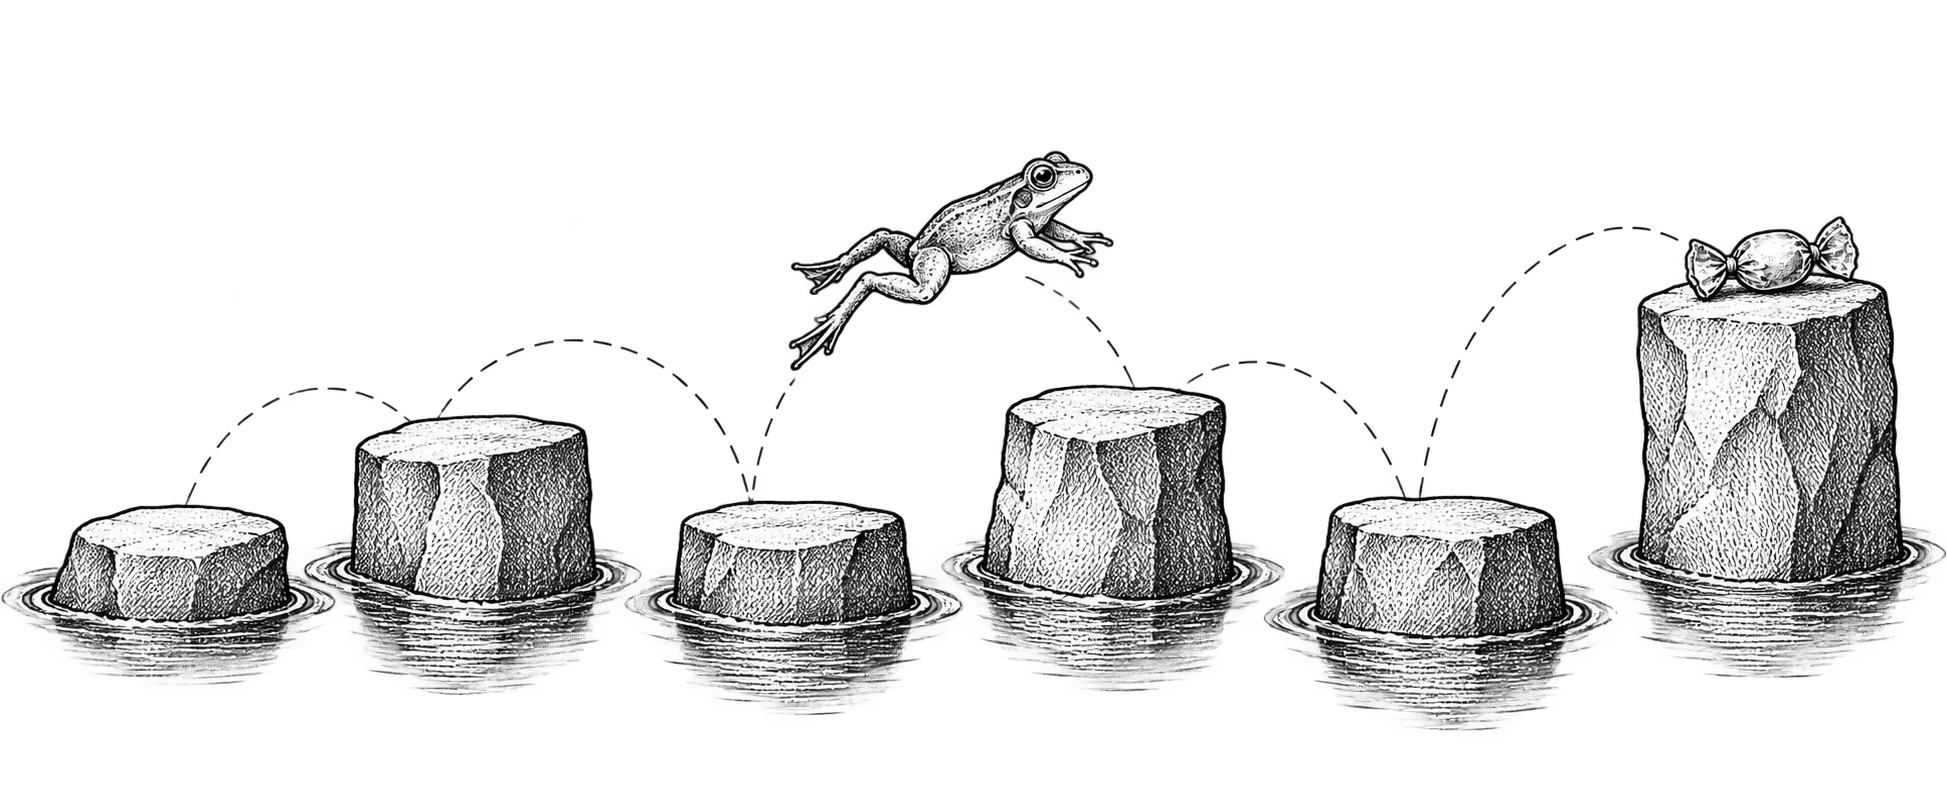
\includegraphics[width=27cm,height=6cm,keepaspectratio]{assets/cover.png}};\node[anchor=west,inner sep=0] at (1.5,1) {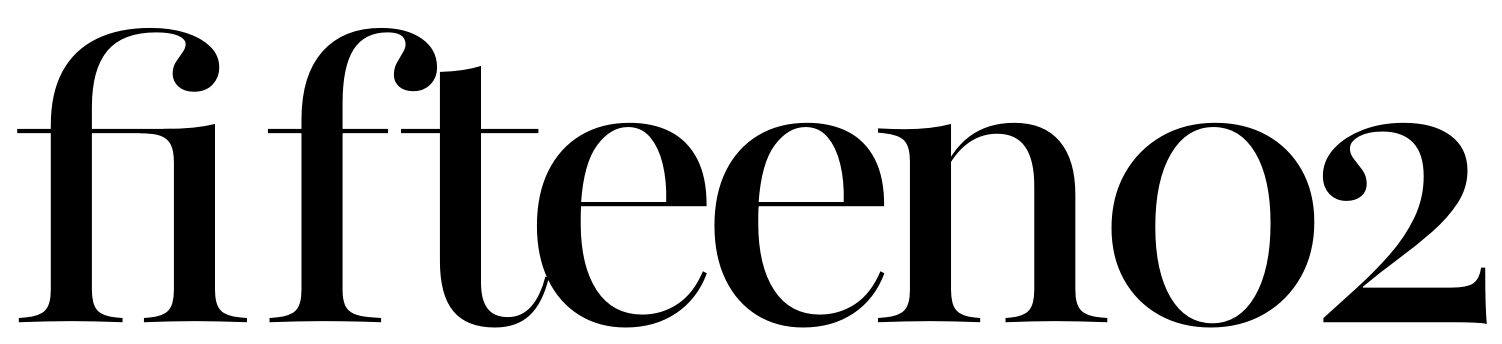
\includegraphics[width=3.8cm]{assets/logo.png}};\node[anchor=east,inner sep=0] at (30.5,1) {
\includegraphics[width=5.5cm]{assets/julians-pathfinder-monochrome.pdf}};
\node[anchor=north west,inner sep=0pt,text width=1cm,align=left,text=quiet,font=\fontsize{11}{\dimexpr11pt*6/5\relax}\selectfont] at (15.8,0.8) {\insertframenumber};
\node[anchor=north west,inner sep=0pt,text width=12cm,align=left,text=ink,font=\fontsize{14}{\dimexpr14pt*6/5\relax}\selectfont] at (18,16.5) {\href{https://colab.research.google.com/github/fifteen02/julians-pathfinder/blob/main/Lesson\%201/lesson.ipynb}{\underline{Open this lesson in Google Colab}}};
\end{scope}\end{tikzpicture}
\end{frame}

\begin{frame}[plain,fragile]\begin{tikzpicture}[remember picture,overlay,x=1cm,y=1cm]\begin{scope}[shift={(current page.south west)}]
\node[anchor=north west,inner sep=0pt,text width=29cm,align=left,text=quiet,font=\fontsize{12}{\dimexpr12pt*6/5\relax}\selectfont] at (1.5,0.8) {Lesson 1 / TODAY};
\node[anchor=north west,inner sep=0pt,text width=1cm,align=left,text=quiet,font=\fontsize{11}{\dimexpr11pt*6/5\relax}\selectfont] at (30,0.8) {\insertframenumber};
\node[anchor=north west,inner sep=0pt,text width=29cm,align=left,text=ink,font=\fontsize{40}{\dimexpr40pt*6/5\relax}\selectfont] at (1.5,16.5) {\heavy Remember the answer.};
\node(idea)[anchor=north west,inner sep=0pt,text width=28cm,align=left,text=ink,font=\fontsize{24}{\dimexpr24pt*6/5\relax}\selectfont] at (1.5,11.9) {When the same question comes up again, reuse its saved answer instead of working it out again.};
\node[anchor=north west,inner sep=0pt,text width=28cm,align=left,font=\fontsize{24}{30}\selectfont] at ([yshift=-9mm]idea.south west) {\textbf{You will be able to}\par\smallskip\hangindent=1.1em\hangafter=1\textbullet\ read a function that calls itself and explain how it stops;\par\hangindent=1.1em\hangafter=1\textbullet\ count staircase routes, then save answers that are needed again;\par\hangindent=1.1em\hangafter=1\textbullet\ solve Frog using exhaustive recursion, caching and an iterative table.\par};
\end{scope}\end{tikzpicture}
\end{frame}

\begin{frame}[plain,fragile]
\begin{tikzpicture}[remember picture,overlay,x=1cm,y=1cm]\begin{scope}[shift={(current page.south west)}]
\node[anchor=north west,inner sep=0pt,text width=29cm,align=left,text=quiet,font=\fontsize{12}{\dimexpr12pt*6/5\relax}\selectfont] at (1.5,0.8) {Lesson 1 / RECURSION};
\node[anchor=north west,inner sep=0pt,text width=1cm,align=left,text=quiet,font=\fontsize{11}{\dimexpr11pt*6/5\relax}\selectfont] at (30,0.8) {\insertframenumber};
\node[anchor=north west,inner sep=0pt,text width=29cm,align=left,text=ink,font=\fontsize{40}{\dimexpr40pt*6/5\relax}\selectfont] at (1.5,16.5) {\heavy A function that calls itself};
\node[anchor=north west,inner sep=0pt,text width=29cm,align=left,text=quiet,font=\fontsize{21}{\dimexpr21pt*6/5\relax}\selectfont] at (1.5,13.0) {\textbf{Objective.} read a function that calls itself and follow what it prints.};
\node(code)[anchor=north west,inner sep=5mm,fill=codepaper,align=left,font=\ttfamily\fontsize{22}{27}\selectfont] at (1.5,11.2) {\textcolor{ink}{def countdown(n):}\\\hspace*{2.4em}\textcolor{ink}{if n == 0:}\\\hspace*{4.8em}\textcolor{returnink}{print('Go!')}\\\hspace*{4.8em}\textcolor{returnink}{return}\\\hspace*{2.4em}\textcolor{ink}{print(n)}\\\hspace*{2.4em}\textcolor{callink}{countdown(n - 1)}};
\node[anchor=north west,inner sep=0pt,text width=13cm,align=left,text=ink,font=\fontsize{22}{\dimexpr22pt*6/5\relax}\selectfont] at (17.5,11.2) {Calling the same function from inside it is \textbf{recursion}. Each call has its own n. Here n is a nonnegative integer.\par\medskip In L1-01, trace countdown(3). Write its output before running it; the answer comes after your attempt.};
\node[anchor=north west,inner sep=0pt,text width=14.5cm,align=left,text=teal,font=\fontsize{20}{\dimexpr20pt*6/5\relax}\selectfont] at (1.5,4.1) {The argument gets smaller at every call, so the calls stop when n reaches 0.};
\end{scope}\end{tikzpicture}
\end{frame}

\begin{frame}[plain,fragile]
\begin{tikzpicture}[remember picture,overlay,x=1cm,y=1cm]\begin{scope}[shift={(current page.south west)}]
\node[anchor=north west,inner sep=0pt,text width=29cm,align=left,text=quiet,font=\fontsize{12}{\dimexpr12pt*6/5\relax}\selectfont] at (1.5,0.8) {Lesson 1 / RECURSION};
\node[anchor=north west,inner sep=0pt,text width=1cm,align=left,text=quiet,font=\fontsize{11}{\dimexpr11pt*6/5\relax}\selectfont] at (30,0.8) {\insertframenumber};
\node[anchor=north west,inner sep=0pt,text width=29cm,align=left,text=ink,font=\fontsize{40}{\dimexpr40pt*6/5\relax}\selectfont] at (1.5,16.5) {\heavy Two parts: a base case and a smaller case};
\node[anchor=north west,inner sep=0pt,text width=29cm,align=left,text=quiet,font=\fontsize{21}{\dimexpr21pt*6/5\relax}\selectfont] at (1.5,13.0) {\textbf{Objective.} name the two parts every recursive function needs.};
\node[anchor=north west,inner sep=0pt,text width=14cm,align=left,text=ink,font=\fontsize{22}{\dimexpr22pt*6/5\relax}\selectfont] at (1.5,11.2) {\textcolor{returnink}{\textbf{Base case:}} an input answered directly, with no further call. In countdown it is n == 0.};
\node[anchor=north west,inner sep=0pt,text width=14cm,align=left,text=ink,font=\fontsize{22}{\dimexpr22pt*6/5\relax}\selectfont] at (16.5,11.2) {\textcolor{callink}{\textbf{Smaller case:}} the function calls itself on a smaller input, which must lead to the base case.};
\begin{scope}[>=Stealth]\node(c0)[draw=callink,line width=1.4pt,rounded corners=3mm,minimum width=5.2cm,minimum height=1.6cm,font=\ttfamily\fontsize{20}{24}\selectfont,fill=callwash] at (6,5.8) {countdown(n)};\node(c1)[draw=callink,line width=1.4pt,rounded corners=3mm,minimum width=5.2cm,minimum height=1.6cm,font=\ttfamily\fontsize{20}{24}\selectfont,fill=callwash] at (18,5.8) {countdown(n - 1)};\draw[->,very thick,callink] (c0)--node[above,font=\fontsize{17}{20}\selectfont]{one smaller input}(c1);\end{scope}
\node[anchor=north west,inner sep=0pt,text width=29cm,align=left,text=ink,font=\fontsize{21}{\dimexpr21pt*6/5\relax}\selectfont] at (1.5,3.2) {The smaller calls must eventually reach n == 0, where countdown makes no further call.};
\end{scope}\end{tikzpicture}
\end{frame}

\begin{frame}[plain,fragile]
\begin{tikzpicture}[remember picture,overlay,x=1cm,y=1cm]\begin{scope}[shift={(current page.south west)}]
\node[anchor=north west,inner sep=0pt,text width=29cm,align=left,text=quiet,font=\fontsize{12}{\dimexpr12pt*6/5\relax}\selectfont] at (1.5,0.8) {Lesson 1 / RECURSION};
\node[anchor=north west,inner sep=0pt,text width=1cm,align=left,text=quiet,font=\fontsize{11}{\dimexpr11pt*6/5\relax}\selectfont] at (30,0.8) {\insertframenumber};
\node[anchor=north west,inner sep=0pt,text width=29cm,align=left,text=ink,font=\fontsize{40}{\dimexpr40pt*6/5\relax}\selectfont] at (1.5,16.5) {\heavy The call stack};
\node[anchor=north west,inner sep=0pt,text width=29cm,align=left,text=quiet,font=\fontsize{21}{\dimexpr21pt*6/5\relax}\selectfont] at (1.5,13.0) {\textbf{Objective.} see why a call waits, and where Python keeps waiting calls.};
\node[anchor=north west,inner sep=0pt,text width=29cm,align=left,text=ink,font=\fontsize{19}{\dimexpr19pt*6/5\relax}\selectfont] at (1.5,11.5) {sum\_to(n) returns 1 + 2 + ... + n; sum\_to(0) returns 0. Data: n = 3.};
\node(code)[anchor=north west,inner sep=5mm,fill=codepaper,align=left,font=\ttfamily\fontsize{22}{27}\selectfont] at (1.5,10.0) {\textcolor{ink}{def sum\_to(n):}\\\hspace*{2.4em}\textcolor{ink}{if n == 0:}\\\hspace*{4.8em}\textcolor{returnink}{return 0}\\\hspace*{2.4em}\textcolor{callink}{return n + sum\_to(n - 1)}};
\node[anchor=north west,inner sep=0pt,text width=14.5cm,align=left,text=ink,font=\fontsize{20}{\dimexpr20pt*6/5\relax}\selectfont] at (1.5,5.0) {\texttt{return} hands a value to the calling function. Python keeps unfinished calls on the \textbf{call stack}. The newest call is on top; the others wait for its answer.};
\node(stack0)[draw=callink,line width=1.4pt,rounded corners=3mm,minimum width=5.2cm,minimum height=1.6cm,font=\ttfamily\fontsize{20}{24}\selectfont,draw=waitink,fill=waitwash,minimum width=7cm] at (21.5,2.2) {sum\_to(3)};\node[anchor=west,font=\fontsize{18}{22}\selectfont,text=quiet] at (25.3,2.2) {waits};
\node(stack1)[draw=callink,line width=1.4pt,rounded corners=3mm,minimum width=5.2cm,minimum height=1.6cm,font=\ttfamily\fontsize{20}{24}\selectfont,draw=waitink,fill=waitwash,minimum width=7cm] at (21.5,4.3) {sum\_to(2)};\node[anchor=west,font=\fontsize{18}{22}\selectfont,text=quiet] at (25.3,4.3) {waits};
\node(stack2)[draw=callink,line width=1.4pt,rounded corners=3mm,minimum width=5.2cm,minimum height=1.6cm,font=\ttfamily\fontsize{20}{24}\selectfont,draw=waitink,fill=waitwash,minimum width=7cm] at (21.5,6.4) {sum\_to(1)};\node[anchor=west,font=\fontsize{18}{22}\selectfont,text=quiet] at (25.3,6.4) {waits};
\node(stack3)[draw=callink,line width=1.4pt,rounded corners=3mm,minimum width=5.2cm,minimum height=1.6cm,font=\ttfamily\fontsize{20}{24}\selectfont,draw=returnink,fill=returnwash,minimum width=7cm] at (21.5,8.5) {sum\_to(0)};\node[anchor=west,font=\fontsize{18}{22}\selectfont,text=quiet] at (25.3,8.5) {returns 0};
\draw[-{Stealth[length=3mm]},callink,line width=2pt] (17.1,2.3)--node[left,rotate=90,anchor=south,font=\fontsize{16}{19}\selectfont]{new calls}(17.1,8.3);\node[font=\fontsize{17}{20}\selectfont,text=returnink] at (21.5,9.8) {top: answer directly};\end{scope}\end{tikzpicture}
\end{frame}

\begin{frame}[plain,fragile]
\begin{tikzpicture}[remember picture,overlay,x=1cm,y=1cm]\begin{scope}[shift={(current page.south west)}]
\node[anchor=north west,inner sep=0pt,text width=29cm,align=left,text=quiet,font=\fontsize{12}{\dimexpr12pt*6/5\relax}\selectfont] at (1.5,0.8) {Lesson 1 / RECURSION / QUESTION};
\node[anchor=north west,inner sep=0pt,text width=1cm,align=left,text=quiet,font=\fontsize{11}{\dimexpr11pt*6/5\relax}\selectfont] at (30,0.8) {\insertframenumber};
\node[anchor=north west,inner sep=0pt,text width=29cm,align=left,text=ink,font=\fontsize{40}{\dimexpr40pt*6/5\relax}\selectfont] at (1.5,16.5) {\heavy Trace sum\_to(3): your turn};
\node[anchor=north west,inner sep=0pt,text width=29cm,align=left,text=quiet,font=\fontsize{21}{\dimexpr21pt*6/5\relax}\selectfont] at (1.5,13.0) {\textbf{Objective.} trace calls down the table, then work out returned values from the bottom up.};
\node(body)[anchor=north west,inner sep=0pt,text width=29cm,align=left,text=ink,font=\fontsize{21}{\dimexpr21pt*6/5\relax}\selectfont] at (1.5,11.2) {Data: n = 3. Fill the missing Returns entries, including each addition. Start with sum\_to(0). Predict the final returned value before going to the next slide.};
\node(trace)[anchor=north west,inner sep=0,text width=26cm] at (3,8.6) {\begingroup\fontsize{20}{24}\selectfont\setlength{\tabcolsep}{5pt}\setlength{\arrayrulewidth}{.5pt}\arrayrulecolor{quiet}\renewcommand{\arraystretch}{1}\begin{tabularx}{\linewidth}{|>{\raggedright\arraybackslash}p{47mm}|>{\centering\arraybackslash}X|>{\centering\arraybackslash}X|}\hline
\rowcolor{wash}\rule[-2.6mm]{0pt}{8mm}\textbf{Call} & \textbf{Waits for} & \textbf{Returns}\\\hline
\rule[-3.4mm]{0pt}{11.5mm}sum\_to(3) & sum\_to(2) & \\\hline
\rule[-3.4mm]{0pt}{11.5mm}sum\_to(2) & sum\_to(1) & \\\hline
\rule[-3.4mm]{0pt}{11.5mm}sum\_to(1) & sum\_to(0) & \\\hline
\rule[-3.4mm]{0pt}{11.5mm}sum\_to(0) & nothing (base case) & 0\\\hline
\end{tabularx}\endgroup};
\draw[-{Stealth[length=3mm]},callink,line width=2pt] (1.7,8)--node[left,rotate=90,anchor=south,font=\fontsize{16}{19}\selectfont]{calls go down}(1.7,4.3);\draw[-{Stealth[length=3mm]},returnink,line width=2pt] (30.3,4.3)--node[right,rotate=90,anchor=north,font=\fontsize{16}{19}\selectfont]{answers come back}(30.3,8);\node[anchor=north west,inner sep=0pt,text width=29cm,align=left,text=teal,font=\fontsize{20}{\dimexpr20pt*6/5\relax}\selectfont] at (1.5,2.4) {Pause here. The next slide contains the completed trace.};
\end{scope}\end{tikzpicture}
\end{frame}

\begin{frame}[plain,fragile]
\begin{tikzpicture}[remember picture,overlay,x=1cm,y=1cm]\begin{scope}[shift={(current page.south west)}]
\node[anchor=north west,inner sep=0pt,text width=29cm,align=left,text=quiet,font=\fontsize{12}{\dimexpr12pt*6/5\relax}\selectfont] at (1.5,0.8) {Lesson 1 / RECURSION / ANSWER};
\node[anchor=north west,inner sep=0pt,text width=1cm,align=left,text=quiet,font=\fontsize{11}{\dimexpr11pt*6/5\relax}\selectfont] at (30,0.8) {\insertframenumber};
\node[anchor=north west,inner sep=0pt,text width=29cm,align=left,text=ink,font=\fontsize{40}{\dimexpr40pt*6/5\relax}\selectfont] at (1.5,16.5) {\heavy Trace sum\_to(3): worked answer};
\node[anchor=north west,inner sep=0pt,text width=29cm,align=left,text=quiet,font=\fontsize{21}{\dimexpr21pt*6/5\relax}\selectfont] at (1.5,13.0) {\textbf{Objective.} trace calls down the table, then work out returned values from the bottom up.};
\node(body)[anchor=north west,inner sep=0pt,text width=29cm,align=left,text=ink,font=\fontsize{21}{\dimexpr21pt*6/5\relax}\selectfont] at (1.5,11.2) {Read the completed Returns column from the bottom up. Each call adds its own n to the result it receives.};
\node(trace)[anchor=north west,inner sep=0,text width=26cm] at (3,8.6) {\begingroup\fontsize{20}{24}\selectfont\setlength{\tabcolsep}{5pt}\setlength{\arrayrulewidth}{.5pt}\arrayrulecolor{quiet}\renewcommand{\arraystretch}{1}\begin{tabularx}{\linewidth}{|>{\raggedright\arraybackslash}p{47mm}|>{\centering\arraybackslash}X|>{\centering\arraybackslash}X|}\hline
\rowcolor{wash}\rule[-2.6mm]{0pt}{8mm}\textbf{Call} & \textbf{Waits for} & \textbf{Returns}\\\hline
\rule[-3.4mm]{0pt}{11.5mm}sum\_to(3) & sum\_to(2) & 3 + 3 = 6\\\hline
\rule[-3.4mm]{0pt}{11.5mm}sum\_to(2) & sum\_to(1) & 2 + 1 = 3\\\hline
\rule[-3.4mm]{0pt}{11.5mm}sum\_to(1) & sum\_to(0) & 1 + 0 = 1\\\hline
\rule[-3.4mm]{0pt}{11.5mm}sum\_to(0) & nothing (base case) & 0\\\hline
\end{tabularx}\endgroup};
\draw[-{Stealth[length=3mm]},callink,line width=2pt] (1.7,8)--node[left,rotate=90,anchor=south,font=\fontsize{16}{19}\selectfont]{calls go down}(1.7,4.3);\draw[-{Stealth[length=3mm]},returnink,line width=2pt] (30.3,4.3)--node[right,rotate=90,anchor=north,font=\fontsize{16}{19}\selectfont]{answers come back}(30.3,8);\node[anchor=north west,inner sep=0pt,text width=29cm,align=left,text=teal,font=\fontsize{20}{\dimexpr20pt*6/5\relax}\selectfont] at (1.5,2.4) {Compare each addition with your prediction before continuing to L1-01.};
\end{scope}\end{tikzpicture}
\end{frame}

\begin{frame}[plain,fragile]\begin{tikzpicture}[remember picture,overlay,x=1cm,y=1cm]\begin{scope}[shift={(current page.south west)}]
\node[anchor=north west,inner sep=0pt,text width=29cm,align=left,text=quiet,font=\fontsize{12}{\dimexpr12pt*6/5\relax}\selectfont] at (1.5,0.8) {Lesson 1 / RECURSION / L1-01 / QUESTION};
\node[anchor=north west,inner sep=0pt,text width=1cm,align=left,text=quiet,font=\fontsize{11}{\dimexpr11pt*6/5\relax}\selectfont] at (30,0.8) {\insertframenumber};
\node[anchor=north west,inner sep=0pt,text width=29cm,align=left,text=ink,font=\fontsize{40}{\dimexpr40pt*6/5\relax}\selectfont] at (1.5,16.5) {\heavy A function that calls itself};
\node(body)[anchor=north west,inner sep=0pt,text width=29cm,align=left,text=ink,font=\fontsize{22}{\dimexpr22pt*6/5\relax}\selectfont] at (1.5,13.0) {A function may call itself on a smaller input. countdown(n) below prints n and then calls countdown(n - 1); when n is 0 it prints Go! and makes no further call. In the table, write every call that countdown(3) makes, in order, what that call prints and which call it makes next.};
\node(given)[anchor=north west,inner sep=3.5mm,fill=codepaper,align=left,font=\ttfamily\fontsize{16}{20}\selectfont] at ([yshift=-7mm,xshift=3.5mm]body.south west) {def countdown(n):\\\hspace*{2.4em}if n == 0:\\\hspace*{4.8em}print('Go!')\\\hspace*{4.8em}return\\\hspace*{2.4em}print(n)\\\hspace*{2.4em}countdown(n - 1)};
\node[anchor=north west,inner sep=0,text width=14cm] at ([xshift=15cm,yshift=-8mm]body.south west) {\begingroup\fontsize{20}{24}\selectfont\setlength{\tabcolsep}{5pt}\setlength{\arrayrulewidth}{.5pt}\arrayrulecolor{quiet}\renewcommand{\arraystretch}{1}\begin{tabularx}{\linewidth}{|>{\raggedright\arraybackslash}p{62mm}|>{\centering\arraybackslash}X|>{\centering\arraybackslash}X|}\hline
\rowcolor{wash}\rule[-2.6mm]{0pt}{8mm}\textbf{Call} & \textbf{Prints} & \textbf{Calls next}\\\hline
\rule[-3.4mm]{0pt}{11.5mm}countdown(3) &  & \\\hline
\rule[-3.4mm]{0pt}{11.5mm} &  & \\\hline
\rule[-3.4mm]{0pt}{11.5mm} &  & \\\hline
\rule[-3.4mm]{0pt}{11.5mm} &  & \\\hline
\end{tabularx}\endgroup};
\end{scope}\end{tikzpicture}
\end{frame}

\begin{frame}[plain,fragile]\begin{tikzpicture}[remember picture,overlay,x=1cm,y=1cm]\begin{scope}[shift={(current page.south west)}]
\node[anchor=north west,inner sep=0pt,text width=29cm,align=left,text=quiet,font=\fontsize{12}{\dimexpr12pt*6/5\relax}\selectfont] at (1.5,0.8) {Lesson 1 / RECURSION / L1-01 / ANSWER};
\node[anchor=north west,inner sep=0pt,text width=1cm,align=left,text=quiet,font=\fontsize{11}{\dimexpr11pt*6/5\relax}\selectfont] at (30,0.8) {\insertframenumber};
\node[anchor=north west,inner sep=0pt,text width=29cm,align=left,text=ink,font=\fontsize{40}{\dimexpr40pt*6/5\relax}\selectfont] at (1.5,16.5) {\heavy A function that calls itself};
\node(body)[anchor=north west,inner sep=0pt,text width=29cm,align=left,text=ink,font=\fontsize{22}{\dimexpr22pt*6/5\relax}\selectfont] at (1.5,13.0) {Read the completed table from top to bottom. Each call prints before making the next call; the base case makes no further call.};
\node(tab)[anchor=north west,inner sep=0,text width=29cm] at ([yshift=-8mm]body.south west) {\begingroup\fontsize{20}{24}\selectfont\setlength{\tabcolsep}{5pt}\setlength{\arrayrulewidth}{.5pt}\arrayrulecolor{quiet}\renewcommand{\arraystretch}{1}\begin{tabularx}{\linewidth}{|>{\raggedright\arraybackslash}p{62mm}|>{\centering\arraybackslash}X|>{\centering\arraybackslash}X|}\hline
\rowcolor{wash}\rule[-2.6mm]{0pt}{8mm}\textbf{Call} & \textbf{Prints} & \textbf{Calls next}\\\hline
\rule[-3.4mm]{0pt}{11.5mm}countdown(3) & 3 & countdown(2)\\\hline
\rule[-3.4mm]{0pt}{11.5mm}countdown(2) & 2 & countdown(1)\\\hline
\rule[-3.4mm]{0pt}{11.5mm}countdown(1) & 1 & countdown(0)\\\hline
\rule[-3.4mm]{0pt}{11.5mm}countdown(0) & Go! & nothing\\\hline
\end{tabularx}\endgroup};
\end{scope}\end{tikzpicture}
\end{frame}

\begin{frame}[plain,fragile]\begin{tikzpicture}[remember picture,overlay,x=1cm,y=1cm]\begin{scope}[shift={(current page.south west)}]
\node[anchor=north west,inner sep=0pt,text width=29cm,align=left,text=quiet,font=\fontsize{12}{\dimexpr12pt*6/5\relax}\selectfont] at (1.5,0.8) {Lesson 1 / RECURSION / L1-02 / QUESTION};
\node[anchor=north west,inner sep=0pt,text width=1cm,align=left,text=quiet,font=\fontsize{11}{\dimexpr11pt*6/5\relax}\selectfont] at (30,0.8) {\insertframenumber};
\node[anchor=north west,inner sep=0pt,text width=29cm,align=left,text=ink,font=\fontsize{40}{\dimexpr40pt*6/5\relax}\selectfont] at (1.5,16.5) {\heavy Wait for the smaller answer};
\node(body)[anchor=north west,inner sep=0pt,text width=29cm,align=left,text=ink,font=\fontsize{22}{\dimexpr22pt*6/5\relax}\selectfont] at (1.5,13.0) {sum\_squares(n) returns 0 when n is 0; otherwise it returns n * n + sum\_squares(n - 1). A call cannot finish until the call it waits for has returned. Fill the table for sum\_squares(4), starting from the bottom row and working up. Write the addition for each returned value.};
\node(given)[anchor=north west,inner sep=3.5mm,fill=codepaper,align=left,font=\ttfamily\fontsize{16}{20}\selectfont] at ([yshift=-7mm,xshift=3.5mm]body.south west) {def sum\_squares(n):\\\hspace*{2.4em}if n == 0:\\\hspace*{4.8em}return 0\\\hspace*{2.4em}return n * n + sum\_squares(n - 1)};
\node[anchor=north west,inner sep=0,text width=14cm] at ([xshift=15cm,yshift=-8mm]body.south west) {\begingroup\fontsize{20}{24}\selectfont\setlength{\tabcolsep}{5pt}\setlength{\arrayrulewidth}{.5pt}\arrayrulecolor{quiet}\renewcommand{\arraystretch}{1}\begin{tabularx}{\linewidth}{|>{\raggedright\arraybackslash}p{73mm}|>{\centering\arraybackslash}X|>{\centering\arraybackslash}X|}\hline
\rowcolor{wash}\rule[-2.6mm]{0pt}{8mm}\textbf{Call} & \textbf{Waits for} & \textbf{Returns}\\\hline
\rule[-3.4mm]{0pt}{10mm}sum\_squares(4) &  & \\\hline
\rule[-3.4mm]{0pt}{10mm}sum\_squares(3) &  & \\\hline
\rule[-3.4mm]{0pt}{10mm}sum\_squares(2) &  & \\\hline
\rule[-3.4mm]{0pt}{10mm}sum\_squares(1) &  & \\\hline
\rule[-3.4mm]{0pt}{10mm}sum\_squares(0) & nothing & 0\\\hline
\end{tabularx}\endgroup};
\end{scope}\end{tikzpicture}
\end{frame}

\begin{frame}[plain,fragile]\begin{tikzpicture}[remember picture,overlay,x=1cm,y=1cm]\begin{scope}[shift={(current page.south west)}]
\node[anchor=north west,inner sep=0pt,text width=29cm,align=left,text=quiet,font=\fontsize{12}{\dimexpr12pt*6/5\relax}\selectfont] at (1.5,0.8) {Lesson 1 / RECURSION / L1-02 / ANSWER};
\node[anchor=north west,inner sep=0pt,text width=1cm,align=left,text=quiet,font=\fontsize{11}{\dimexpr11pt*6/5\relax}\selectfont] at (30,0.8) {\insertframenumber};
\node[anchor=north west,inner sep=0pt,text width=29cm,align=left,text=ink,font=\fontsize{40}{\dimexpr40pt*6/5\relax}\selectfont] at (1.5,16.5) {\heavy Wait for the smaller answer};
\node(body)[anchor=north west,inner sep=0pt,text width=29cm,align=left,text=ink,font=\fontsize{22}{\dimexpr22pt*6/5\relax}\selectfont] at (1.5,13.0) {Fill the returned values from the bottom row upward. Each call adds its own square to the value returned by the next row.};
\node(tab)[anchor=north west,inner sep=0,text width=29cm] at ([yshift=-8mm]body.south west) {\begingroup\fontsize{20}{24}\selectfont\setlength{\tabcolsep}{5pt}\setlength{\arrayrulewidth}{.5pt}\arrayrulecolor{quiet}\renewcommand{\arraystretch}{1}\begin{tabularx}{\linewidth}{|>{\raggedright\arraybackslash}p{73mm}|>{\centering\arraybackslash}X|>{\centering\arraybackslash}X|}\hline
\rowcolor{wash}\rule[-2.6mm]{0pt}{8mm}\textbf{Call} & \textbf{Waits for} & \textbf{Returns}\\\hline
\rule[-3.4mm]{0pt}{10mm}sum\_squares(4) & sum\_squares(3) & 16 + 14 = 30\\\hline
\rule[-3.4mm]{0pt}{10mm}sum\_squares(3) & sum\_squares(2) & 9 + 5 = 14\\\hline
\rule[-3.4mm]{0pt}{10mm}sum\_squares(2) & sum\_squares(1) & 4 + 1 = 5\\\hline
\rule[-3.4mm]{0pt}{10mm}sum\_squares(1) & sum\_squares(0) & 1 + 0 = 1\\\hline
\rule[-3.4mm]{0pt}{10mm}sum\_squares(0) & nothing & 0\\\hline
\end{tabularx}\endgroup};
\end{scope}\end{tikzpicture}
\end{frame}

\begin{frame}[plain,fragile]\begin{tikzpicture}[remember picture,overlay,x=1cm,y=1cm]\begin{scope}[shift={(current page.south west)}]
\node[anchor=north west,inner sep=0pt,text width=29cm,align=left,text=quiet,font=\fontsize{12}{\dimexpr12pt*6/5\relax}\selectfont] at (1.5,0.8) {Lesson 1 / RECURSION / L1-03 / QUESTION};
\node[anchor=north west,inner sep=0pt,text width=1cm,align=left,text=quiet,font=\fontsize{11}{\dimexpr11pt*6/5\relax}\selectfont] at (30,0.8) {\insertframenumber};
\node[anchor=north west,inner sep=0pt,text width=29cm,align=left,text=ink,font=\fontsize{40}{\dimexpr40pt*6/5\relax}\selectfont] at (1.5,16.5) {\heavy Find the missing base case};
\node(body)[anchor=north west,inner sep=0pt,text width=29cm,align=left,text=ink,font=\fontsize{20}{\dimexpr20pt*6/5\relax}\selectfont] at (1.5,13.0) {power2(n) below should return 2 to the power n: 2 multiplied by itself n times, so power2(3) should be 8. What happens when you call power2(3)? Which value of n can you answer directly, without a smaller call? Add that base case and check that power2(3) now returns 8.};
\node(given)[anchor=north west,inner sep=3.5mm,fill=codepaper,align=left,font=\ttfamily\fontsize{16}{20}\selectfont] at ([yshift=-7mm,xshift=3.5mm]body.south west) {def power2(n):\\\hspace*{2.4em}return 2 * power2(n - 1)};
\node(sig)[anchor=north west,inner sep=3mm,fill=codepaper,align=left,font=\ttfamily\fontsize{16}{20}\selectfont] at ([yshift=-4mm,xshift=3mm]given.south west) {def power2(n):\\\hspace*{2.4em}return None  \# Replace this};
\node(result)[anchor=north west,inner sep=0pt,text width=13.5cm,align=left,text=quiet,font=\fontsize{17}{20}\selectfont] at ([yshift=-4mm,xshift=15.5cm]given.south west) {\textbf{Returns}\par \textbf{power2(n)}: the integer 2 raised to the power n.\par\smallskip };
\node(both)[fit=(sig)(result),inner sep=0] {};
\node[anchor=north west,inner sep=0pt,text width=29cm,align=left,text=quiet,font=\fontsize{18}{22}\selectfont] at ([yshift=-3mm,xshift=-3mm]both.south west) {\textbf{Hints.} Trace the inputs until they pass 0. Where should the chain stop? Check your repaired function on the stopping input before trying 3.};
\end{scope}\end{tikzpicture}
\end{frame}

\begin{frame}[plain,fragile]\begin{tikzpicture}[remember picture,overlay,x=1cm,y=1cm]\begin{scope}[shift={(current page.south west)}]
\node[anchor=north west,inner sep=0pt,text width=29cm,align=left,text=quiet,font=\fontsize{12}{\dimexpr12pt*6/5\relax}\selectfont] at (1.5,0.8) {Lesson 1 / RECURSION / L1-03 / ANSWER};
\node[anchor=north west,inner sep=0pt,text width=1cm,align=left,text=quiet,font=\fontsize{11}{\dimexpr11pt*6/5\relax}\selectfont] at (30,0.8) {\insertframenumber};
\node[anchor=north west,inner sep=0pt,text width=29cm,align=left,text=ink,font=\fontsize{40}{\dimexpr40pt*6/5\relax}\selectfont] at (1.5,16.5) {\heavy Find the missing base case};
\node(body)[anchor=north west,inner sep=0pt,text width=29cm,align=left,text=ink,font=\fontsize{22}{\dimexpr22pt*6/5\relax}\selectfont] at (1.5,13.0) {The incomplete version continues past input 0 until Python raises RecursionError. Check n == 0 before the smaller call and return 1 there. The completed trace below uses that stopping case.};
\node(tab)[anchor=north west,inner sep=0,text width=29cm] at ([yshift=-8mm]body.south west) {\begingroup\fontsize{20}{24}\selectfont\setlength{\tabcolsep}{5pt}\setlength{\arrayrulewidth}{.5pt}\arrayrulecolor{quiet}\renewcommand{\arraystretch}{1}\begin{tabularx}{\linewidth}{|>{\raggedright\arraybackslash}p{47mm}|>{\centering\arraybackslash}X|>{\centering\arraybackslash}X|}\hline
\rowcolor{wash}\rule[-2.6mm]{0pt}{8mm}\textbf{Call} & \textbf{Waits for} & \textbf{Returns}\\\hline
\rule[-3.4mm]{0pt}{11.5mm}power2(3) & power2(2) & 2 x 4 = 8\\\hline
\rule[-3.4mm]{0pt}{11.5mm}power2(2) & power2(1) & 2 x 2 = 4\\\hline
\rule[-3.4mm]{0pt}{11.5mm}power2(1) & power2(0) & 2 x 1 = 2\\\hline
\rule[-3.4mm]{0pt}{11.5mm}power2(0) & nothing & 1\\\hline
\end{tabularx}\endgroup};
\end{scope}\end{tikzpicture}
\end{frame}

\begin{frame}[plain,fragile]
\begin{lrbox}{\codebox}\begin{minipage}{433pt}
\begin{lstlisting}[basicstyle=\ttfamily\fontsize{24.0}{26.9}\selectfont\color{ink},numbers=left,numberstyle=\ttfamily\fontsize{15.6}{26.9}\selectfont\color{quiet},numbersep=12pt,xleftmargin=23pt,firstnumber=1,breaklines=false,aboveskip=0pt,belowskip=0pt]
def power2(n):
    if n == 0:
        return 1
    return 2 * power2(n - 1)
\end{lstlisting}
\end{minipage}\end{lrbox}
\begin{tikzpicture}[remember picture,overlay,x=1cm,y=1cm]\begin{scope}[shift={(current page.south west)}]
\node[anchor=north west,inner sep=0pt,text width=29cm,align=left,text=quiet,font=\fontsize{12}{\dimexpr12pt*6/5\relax}\selectfont] at (1.5,0.8) {Lesson 1 / RECURSION / L1-03 / ANSWER: PYTHON};
\node[anchor=north west,inner sep=0pt,text width=1cm,align=left,text=quiet,font=\fontsize{11}{\dimexpr11pt*6/5\relax}\selectfont] at (30,0.8) {\insertframenumber};
\node[anchor=north west,inner sep=0pt,text width=29cm,align=left,text=ink,font=\fontsize{40}{48}\selectfont] at (1.5,16.5) {\heavy power2(n)};
\node[anchor=north,inner sep=5mm,fill=codepaper] at (16,13.0) {\usebox{\codebox}};
\end{scope}\end{tikzpicture}

\end{frame}

\begin{frame}[plain,fragile]\begin{tikzpicture}[remember picture,overlay,x=1cm,y=1cm]\begin{scope}[shift={(current page.south west)}]
\node[anchor=north west,inner sep=0pt,text width=29cm,align=left,text=quiet,font=\fontsize{12}{\dimexpr12pt*6/5\relax}\selectfont] at (1.5,0.8) {Lesson 1 / RECURSION / L1-04 / QUESTION};
\node[anchor=north west,inner sep=0pt,text width=1cm,align=left,text=quiet,font=\fontsize{11}{\dimexpr11pt*6/5\relax}\selectfont] at (30,0.8) {\insertframenumber};
\node[anchor=north west,inner sep=0pt,text width=29cm,align=left,text=ink,font=\fontsize{40}{\dimexpr40pt*6/5\relax}\selectfont] at (1.5,16.5) {\heavy Write a recursive function};
\node(body)[anchor=north west,inner sep=0pt,text width=29cm,align=left,text=ink,font=\fontsize{20}{\dimexpr20pt*6/5\relax}\selectfont] at (1.5,13.0) {factorial(n) is the product 1 × 2 × ... × n, and factorial(0) is 1. Write factorial(n) recursively: first the base case, then one smaller call. Predict factorial(4) before running it. The staircase that follows uses the same pattern, with two smaller calls instead of one.};
\node(sig)[anchor=north west,inner sep=3mm,fill=codepaper,align=left,font=\ttfamily\fontsize{16}{20}\selectfont] at ([yshift=-4mm,xshift=3mm]body.south west) {def factorial(n):\\\hspace*{2.4em}return None  \# Replace this};
\node(result)[anchor=north west,inner sep=0pt,text width=13.5cm,align=left,text=quiet,font=\fontsize{17}{20}\selectfont] at ([yshift=-4mm,xshift=15.5cm]body.south west) {\textbf{Returns}\par \textbf{factorial(n)}: the product of integers 1 through n; for n = 0, return 1.\par\smallskip };
\node(both)[fit=(sig)(result),inner sep=0] {};
\node[anchor=north west,inner sep=0pt,text width=29cm,align=left,text=quiet,font=\fontsize{18}{22}\selectfont] at ([yshift=-3mm,xshift=-3mm]both.south west) {\textbf{Hints.} What is the smallest n you can answer directly? If you already knew factorial(n - 1), what single step would give factorial(n)?};
\end{scope}\end{tikzpicture}
\end{frame}

\begin{frame}[plain,fragile]\begin{tikzpicture}[remember picture,overlay,x=1cm,y=1cm]\begin{scope}[shift={(current page.south west)}]
\node[anchor=north west,inner sep=0pt,text width=29cm,align=left,text=quiet,font=\fontsize{12}{\dimexpr12pt*6/5\relax}\selectfont] at (1.5,0.8) {Lesson 1 / RECURSION / L1-04 / ANSWER};
\node[anchor=north west,inner sep=0pt,text width=1cm,align=left,text=quiet,font=\fontsize{11}{\dimexpr11pt*6/5\relax}\selectfont] at (30,0.8) {\insertframenumber};
\node[anchor=north west,inner sep=0pt,text width=29cm,align=left,text=ink,font=\fontsize{40}{\dimexpr40pt*6/5\relax}\selectfont] at (1.5,16.5) {\heavy Write a recursive function};
\node(body)[anchor=north west,inner sep=0pt,text width=29cm,align=left,text=ink,font=\fontsize{22}{\dimexpr22pt*6/5\relax}\selectfont] at (1.5,13.0) {Return 1 at input 0. For a positive input, multiply that input by the result of the call with input one smaller. The table shows the returned values.};
\node(tab)[anchor=north west,inner sep=0,text width=29cm] at ([yshift=-8mm]body.south west) {\begingroup\fontsize{20}{24}\selectfont\setlength{\tabcolsep}{5pt}\setlength{\arrayrulewidth}{.5pt}\arrayrulecolor{quiet}\renewcommand{\arraystretch}{1}\begin{tabularx}{\linewidth}{|>{\raggedright\arraybackslash}p{62mm}|>{\centering\arraybackslash}X|>{\centering\arraybackslash}X|}\hline
\rowcolor{wash}\rule[-2.6mm]{0pt}{8mm}\textbf{Call} & \textbf{Waits for} & \textbf{Returns}\\\hline
\rule[-3.4mm]{0pt}{10mm}factorial(4) & factorial(3) & 4 x 6 = 24\\\hline
\rule[-3.4mm]{0pt}{10mm}factorial(3) & factorial(2) & 3 x 2 = 6\\\hline
\rule[-3.4mm]{0pt}{10mm}factorial(2) & factorial(1) & 2 x 1 = 2\\\hline
\rule[-3.4mm]{0pt}{10mm}factorial(1) & factorial(0) & 1 x 1 = 1\\\hline
\rule[-3.4mm]{0pt}{10mm}factorial(0) & nothing & 1\\\hline
\end{tabularx}\endgroup};
\end{scope}\end{tikzpicture}
\end{frame}

\begin{frame}[plain,fragile]
\begin{lrbox}{\codebox}\begin{minipage}{476pt}
\begin{lstlisting}[basicstyle=\ttfamily\fontsize{24.0}{26.9}\selectfont\color{ink},numbers=left,numberstyle=\ttfamily\fontsize{15.6}{26.9}\selectfont\color{quiet},numbersep=12pt,xleftmargin=23pt,firstnumber=1,breaklines=false,aboveskip=0pt,belowskip=0pt]
def factorial(n):
    if n == 0:
        return 1
    return n * factorial(n - 1)
\end{lstlisting}
\end{minipage}\end{lrbox}
\begin{tikzpicture}[remember picture,overlay,x=1cm,y=1cm]\begin{scope}[shift={(current page.south west)}]
\node[anchor=north west,inner sep=0pt,text width=29cm,align=left,text=quiet,font=\fontsize{12}{\dimexpr12pt*6/5\relax}\selectfont] at (1.5,0.8) {Lesson 1 / RECURSION / L1-04 / ANSWER: PYTHON};
\node[anchor=north west,inner sep=0pt,text width=1cm,align=left,text=quiet,font=\fontsize{11}{\dimexpr11pt*6/5\relax}\selectfont] at (30,0.8) {\insertframenumber};
\node[anchor=north west,inner sep=0pt,text width=29cm,align=left,text=ink,font=\fontsize{40}{48}\selectfont] at (1.5,16.5) {\heavy factorial(n)};
\node[anchor=north,inner sep=5mm,fill=codepaper] at (16,13.0) {\usebox{\codebox}};
\end{scope}\end{tikzpicture}

\end{frame}

\begin{frame}[plain,fragile]\begin{tikzpicture}[remember picture,overlay,x=1cm,y=1cm]\begin{scope}[shift={(current page.south west)}]
\node[anchor=north west,inner sep=0pt,text width=29cm,align=left,text=ink,font=\fontsize{40}{\dimexpr40pt*6/5\relax}\selectfont] at (1.5,16.5) {\heavy From one call to many routes};
\node[anchor=north west,inner sep=0pt,text width=29cm,align=left,text=ink,font=\fontsize{24}{\dimexpr24pt*6/5\relax}\selectfont] at (1.5,13) {We can now follow a recursive call and see where it stops. Next, use calls to count the routes up a staircase.};
\node[anchor=north west,inner sep=0pt,text width=8.5cm,align=left,text=callink,font=\fontsize{25}{\dimexpr25pt*6/5\relax}\selectfont] at (1.5,9.4) {\textbf{1. Explore}};
\node[anchor=north west,inner sep=0pt,text width=8.5cm,align=left,text=ink,font=\fontsize{21}{\dimexpr21pt*6/5\relax}\selectfont] at (1.5,7.8) {Explore the possible last moves with recursive calls.};
\draw[-{Stealth[length=3mm]},quiet,line width=1pt] (10.0,8.9)--(10.8,8.9);
\node[anchor=north west,inner sep=0pt,text width=8.5cm,align=left,text=waitink,font=\fontsize{25}{\dimexpr25pt*6/5\relax}\selectfont] at (11.5,9.4) {\textbf{2. Remember}};
\node[anchor=north west,inner sep=0pt,text width=8.5cm,align=left,text=ink,font=\fontsize{21}{\dimexpr21pt*6/5\relax}\selectfont] at (11.5,7.8) {Save answers so repeated calls do not repeat the work.};
\draw[-{Stealth[length=3mm]},quiet,line width=1pt] (20.0,8.9)--(20.8,8.9);
\node[anchor=north west,inner sep=0pt,text width=8.5cm,align=left,text=returnink,font=\fontsize{25}{\dimexpr25pt*6/5\relax}\selectfont] at (21.5,9.4) {\textbf{3. Build in order}};
\node[anchor=north west,inner sep=0pt,text width=8.5cm,align=left,text=ink,font=\fontsize{21}{\dimexpr21pt*6/5\relax}\selectfont] at (21.5,7.8) {Fill earlier answers first, then use them for later steps.};
\node[anchor=south,inner sep=0] at (16,1.6) {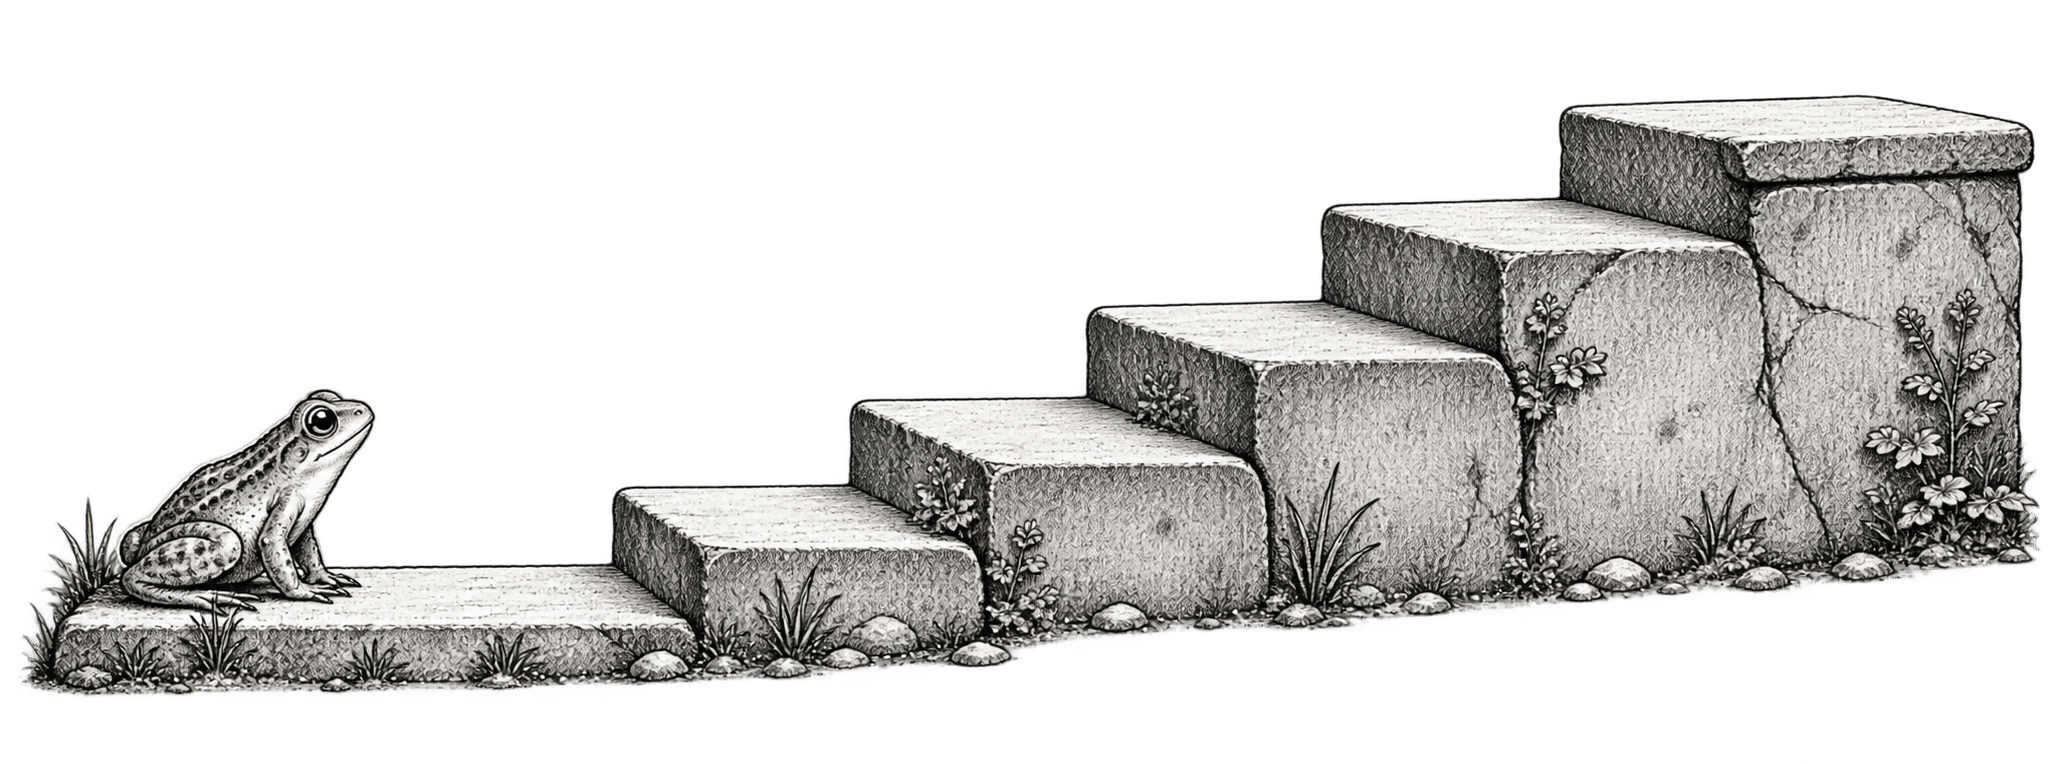
\includegraphics[width=18cm,height=3.6cm,keepaspectratio]{assets/slides/staircase.png}};
\node[anchor=north west,inner sep=0pt,text width=28cm,align=left,text=quiet,font=\fontsize{12}{\dimexpr12pt*6/5\relax}\selectfont] at (1.5,0.8) {Lesson 1 / STAIRCASE / OUR NEXT QUESTION};
\node[anchor=north west,inner sep=0pt,text width=1cm,align=left,text=quiet,font=\fontsize{11}{\dimexpr11pt*6/5\relax}\selectfont] at (30,0.8) {\insertframenumber};
\end{scope}\end{tikzpicture}
\end{frame}

\begin{frame}[plain,fragile]\begin{tikzpicture}[remember picture,overlay,x=1cm,y=1cm]\begin{scope}[shift={(current page.south west)}]
\node[anchor=north west,inner sep=0pt,text width=29cm,align=left,text=quiet,font=\fontsize{12}{\dimexpr12pt*6/5\relax}\selectfont] at (1.5,0.8) {Lesson 1 / STAIRCASE / L1-05 / QUESTION};
\node[anchor=north west,inner sep=0pt,text width=1cm,align=left,text=quiet,font=\fontsize{11}{\dimexpr11pt*6/5\relax}\selectfont] at (30,0.8) {\insertframenumber};
\node[anchor=north west,inner sep=0pt,text width=29cm,align=left,text=ink,font=\fontsize{40}{\dimexpr40pt*6/5\relax}\selectfont] at (1.5,16.5) {\heavy Five steps, many routes};
\node(body)[anchor=north west,inner sep=0pt,text width=29cm,align=left,text=ink,font=\fontsize{23}{\dimexpr23pt*6/5\relax}\selectfont] at (1.5,13.0) {Start on the ground, called step 0. Each move climbs exactly 1 or 2 steps. Count routes that land exactly on each target from step 1 to step 5. List the routes to step 5 as move lists, such as [1, 2, 2]. Does changing the order make a different route?};
\node[anchor=north west,inner sep=0,text width=29cm] at ([yshift=-8mm]body.south west) {\begingroup\fontsize{22}{26}\selectfont\setlength{\tabcolsep}{5pt}\setlength{\arrayrulewidth}{.5pt}\arrayrulecolor{quiet}\renewcommand{\arraystretch}{1}\begin{tabularx}{\linewidth}{|>{\raggedright\arraybackslash}p{34mm}|>{\centering\arraybackslash}X|>{\centering\arraybackslash}X|>{\centering\arraybackslash}X|>{\centering\arraybackslash}X|>{\centering\arraybackslash}X|}\hline
\rowcolor{wash}\rule[-3mm]{0pt}{9.5mm}\textbf{Step} & \textbf{1} & \textbf{2} & \textbf{3} & \textbf{4} & \textbf{5}\\\hline
\rule[-4.6mm]{0pt}{13.5mm}Routes &  &  &  &  & \\\hline
\end{tabularx}\endgroup};
\node[anchor=south,inner sep=0] at (16,1.3) {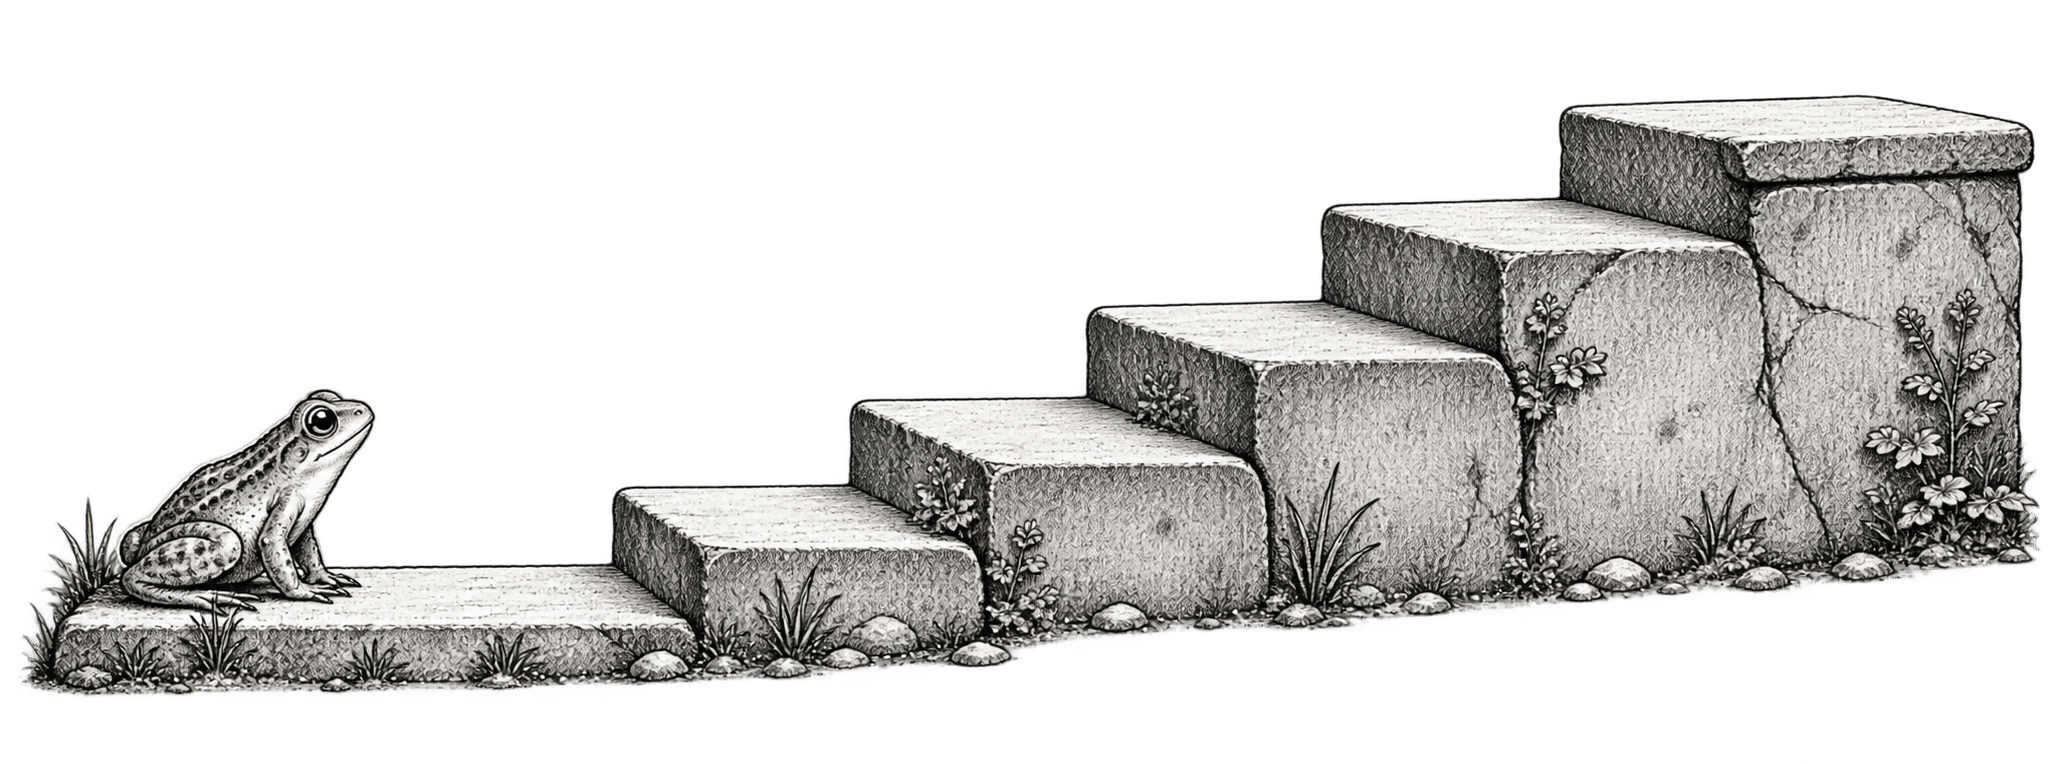
\includegraphics[width=24cm,height=3.8cm,keepaspectratio]{assets/slides/staircase.png}};
\end{scope}\end{tikzpicture}
\end{frame}

\begin{frame}[plain,fragile]\begin{tikzpicture}[remember picture,overlay,x=1cm,y=1cm]\begin{scope}[shift={(current page.south west)}]
\node[anchor=north west,inner sep=0pt,text width=29cm,align=left,text=quiet,font=\fontsize{12}{\dimexpr12pt*6/5\relax}\selectfont] at (1.5,0.8) {Lesson 1 / STAIRCASE / L1-05 / ANSWER};
\node[anchor=north west,inner sep=0pt,text width=1cm,align=left,text=quiet,font=\fontsize{11}{\dimexpr11pt*6/5\relax}\selectfont] at (30,0.8) {\insertframenumber};
\node[anchor=north west,inner sep=0pt,text width=29cm,align=left,text=ink,font=\fontsize{40}{\dimexpr40pt*6/5\relax}\selectfont] at (1.5,16.5) {\heavy Five steps, many routes};
\node(body)[anchor=north west,inner sep=0pt,text width=29cm,align=left,text=ink,font=\fontsize{22}{\dimexpr22pt*6/5\relax}\selectfont] at (1.5,13.0) {Steps 1 through 5 have 1, 2, 3, 5 and 8 routes. The routes to step 5 are 11111, 1112, 1121, 1211, 2111, 122, 212, 221. Each digit is one move. Order matters: 122 and 212 visit different steps.};
\node(tab)[anchor=north west,inner sep=0,text width=29cm] at ([yshift=-8mm]body.south west) {\begingroup\fontsize{22}{26}\selectfont\setlength{\tabcolsep}{5pt}\setlength{\arrayrulewidth}{.5pt}\arrayrulecolor{quiet}\renewcommand{\arraystretch}{1}\begin{tabularx}{\linewidth}{|>{\raggedright\arraybackslash}p{34mm}|>{\centering\arraybackslash}X|>{\centering\arraybackslash}X|>{\centering\arraybackslash}X|>{\centering\arraybackslash}X|>{\centering\arraybackslash}X|}\hline
\rowcolor{wash}\rule[-3mm]{0pt}{9.5mm}\textbf{Step} & \textbf{1} & \textbf{2} & \textbf{3} & \textbf{4} & \textbf{5}\\\hline
\rule[-4.6mm]{0pt}{13.5mm}Routes & 1 & 2 & 3 & 5 & 8\\\hline
\end{tabularx}\endgroup};
\end{scope}\end{tikzpicture}
\end{frame}

\begin{frame}[plain,fragile]\begin{tikzpicture}[remember picture,overlay,x=1cm,y=1cm]\begin{scope}[shift={(current page.south west)}]
\node[anchor=north west,inner sep=0pt,text width=29cm,align=left,text=quiet,font=\fontsize{12}{\dimexpr12pt*6/5\relax}\selectfont] at (1.5,0.8) {Lesson 1 / STAIRCASE / L1-06 / QUESTION};
\node[anchor=north west,inner sep=0pt,text width=1cm,align=left,text=quiet,font=\fontsize{11}{\dimexpr11pt*6/5\relax}\selectfont] at (30,0.8) {\insertframenumber};
\node[anchor=north west,inner sep=0pt,text width=29cm,align=left,text=ink,font=\fontsize{40}{\dimexpr40pt*6/5\relax}\selectfont] at (1.5,16.5) {\heavy The last move explains the sum};
\node(body)[anchor=north west,inner sep=0pt,text width=29cm,align=left,text=ink,font=\fontsize{22}{\dimexpr22pt*6/5\relax}\selectfont] at (1.5,13.0) {The next move must land on step 5. Where can that move start? Use your L1-05 counts for step 4 and step 3. How can these two counts give the answer for step 5?};
\node[anchor=north west,inner sep=0,text width=28cm] at (1.5,6.5) {\resizebox{18cm}{!}{\begin{minipage}{14cm}\begin{center}\begin{tikzpicture}[>=Stealth,every node/.style={font=\fontsize{13}{15}\selectfont},box/.style={draw=teal,rounded corners,minimum width=20mm,minimum height=8mm,fill=wash},arr/.style={->,thick,teal}]\node[box] (a) at (0,1) {step ?};\node[box] (b) at (0,-1) {step ?};\node[box] (c) at (8,0) {step 5};\draw[arr] (a)--node[above,sloped]{final jump of 1}(c);\draw[arr] (b)--node[below,sloped]{final jump of 2}(c);\end{tikzpicture}\end{center}\end{minipage}}};
\end{scope}\end{tikzpicture}
\end{frame}

\begin{frame}[plain,fragile]\begin{tikzpicture}[remember picture,overlay,x=1cm,y=1cm]\begin{scope}[shift={(current page.south west)}]
\node[anchor=north west,inner sep=0pt,text width=29cm,align=left,text=quiet,font=\fontsize{12}{\dimexpr12pt*6/5\relax}\selectfont] at (1.5,0.8) {Lesson 1 / STAIRCASE / L1-06 / ANSWER};
\node[anchor=north west,inner sep=0pt,text width=1cm,align=left,text=quiet,font=\fontsize{11}{\dimexpr11pt*6/5\relax}\selectfont] at (30,0.8) {\insertframenumber};
\node[anchor=north west,inner sep=0pt,text width=29cm,align=left,text=ink,font=\fontsize{40}{\dimexpr40pt*6/5\relax}\selectfont] at (1.5,16.5) {\heavy The last move explains the sum};
\node(body)[anchor=north west,inner sep=0pt,text width=29cm,align=left,text=ink,font=\fontsize{22}{\dimexpr22pt*6/5\relax}\selectfont] at (1.5,13.0) {The last move starts at step 4 with a jump of 1, or at step 3 with a jump of 2. Extend each earlier route once. The groups cannot overlap because their last moves differ: 5 + 3 = 8.};
\node[anchor=north west,inner sep=0,text width=28cm] at (1.5,6.5) {\resizebox{18cm}{!}{\begin{minipage}{14cm}\begin{center}\begin{tikzpicture}[>=Stealth,every node/.style={font=\fontsize{13}{15}\selectfont},box/.style={draw=teal,rounded corners,minimum width=20mm,minimum height=8mm,fill=wash},arr/.style={->,thick,teal}]\node[box] (a) at (0,1) {step 4};\node[box] (b) at (0,-1) {step 3};\node[box] (c) at (8,0) {step 5};\draw[arr] (a)--node[above,sloped]{5 routes, then jump 1}(c);\draw[arr] (b)--node[below,sloped]{3 routes, then jump 2}(c);\end{tikzpicture}\end{center}\end{minipage}}};
\end{scope}\end{tikzpicture}
\end{frame}

\begin{frame}[plain,fragile]\begin{tikzpicture}[remember picture,overlay,x=1cm,y=1cm]\begin{scope}[shift={(current page.south west)}]
\node[anchor=north west,inner sep=0pt,text width=29cm,align=left,text=quiet,font=\fontsize{12}{\dimexpr12pt*6/5\relax}\selectfont] at (1.5,0.8) {Lesson 1 / STAIRCASE / L1-07 / QUESTION};
\node[anchor=north west,inner sep=0pt,text width=1cm,align=left,text=quiet,font=\fontsize{11}{\dimexpr11pt*6/5\relax}\selectfont] at (30,0.8) {\insertframenumber};
\node[anchor=north west,inner sep=0pt,text width=29cm,align=left,text=ink,font=\fontsize{40}{\dimexpr40pt*6/5\relax}\selectfont] at (1.5,16.5) {\heavy Where recursion stops};
\node(body)[anchor=north west,inner sep=0pt,text width=29cm,align=left,text=ink,font=\fontsize{25}{\dimexpr25pt*6/5\relax}\selectfont] at (1.5,13.0) {Let ways(n) return the number of routes from the ground to target step n, using jumps of 1 or 2. What should ways(0) and ways(-1) return? Use these answers to work out ways(1).};
\node[anchor=north west,inner sep=0pt,text width=28cm,align=left,text=quiet,font=\fontsize{22}{\dimexpr22pt*6/5\relax}\selectfont] at (1.5,4.0) {Think on your own first. Then compare your reasoning with a partner.};
\end{scope}\end{tikzpicture}
\end{frame}

\begin{frame}[plain,fragile]\begin{tikzpicture}[remember picture,overlay,x=1cm,y=1cm]\begin{scope}[shift={(current page.south west)}]
\node[anchor=north west,inner sep=0pt,text width=29cm,align=left,text=quiet,font=\fontsize{12}{\dimexpr12pt*6/5\relax}\selectfont] at (1.5,0.8) {Lesson 1 / STAIRCASE / L1-07 / ANSWER};
\node[anchor=north west,inner sep=0pt,text width=1cm,align=left,text=quiet,font=\fontsize{11}{\dimexpr11pt*6/5\relax}\selectfont] at (30,0.8) {\insertframenumber};
\node[anchor=north west,inner sep=0pt,text width=29cm,align=left,text=ink,font=\fontsize{40}{\dimexpr40pt*6/5\relax}\selectfont] at (1.5,16.5) {\heavy Where recursion stops};
\node(body)[anchor=north west,inner sep=0pt,text width=29cm,align=left,text=ink,font=\fontsize{25}{\dimexpr25pt*6/5\relax}\selectfont] at (1.5,13.0) {ways(0) = 1: the empty list is one way to climb zero steps. ways(-1) = 0: positive jumps cannot finish below the ground. Therefore ways(1) = ways(0) + ways(-1) = 1.};
\node[anchor=north west,inner sep=0pt,text width=28cm,align=left,text=quiet,font=\fontsize{21}{\dimexpr21pt*6/5\relax}\selectfont] at (1.5,4.0) {\textbf{Watch for:} Returning zero for ways(0) makes every later count zero.};
\end{scope}\end{tikzpicture}
\end{frame}

\begin{frame}[plain,fragile]\begin{tikzpicture}[remember picture,overlay,x=1cm,y=1cm]\begin{scope}[shift={(current page.south west)}]
\node[anchor=north west,inner sep=0pt,text width=29cm,align=left,text=quiet,font=\fontsize{12}{\dimexpr12pt*6/5\relax}\selectfont] at (1.5,0.8) {Lesson 1 / STAIRCASE / L1-08 / QUESTION};
\node[anchor=north west,inner sep=0pt,text width=1cm,align=left,text=quiet,font=\fontsize{11}{\dimexpr11pt*6/5\relax}\selectfont] at (30,0.8) {\insertframenumber};
\node[anchor=north west,inner sep=0pt,text width=29cm,align=left,text=ink,font=\fontsize{40}{\dimexpr40pt*6/5\relax}\selectfont] at (1.5,16.5) {\heavy The slow recursive program};
\node(body)[anchor=north west,inner sep=0pt,text width=29cm,align=left,text=ink,font=\fontsize{20}{\dimexpr20pt*6/5\relax}\selectfont] at (1.5,13.0) {Write stairs\_slow(n), the number of staircase routes to step n with jumps of 1 or 2. Start with the stopping cases, then ask about the two possible starting steps of the final jump. Draw every call made for stairs\_slow(3) and write the returned count beside it.};
\node(sig)[anchor=north west,inner sep=3mm,fill=codepaper,align=left,font=\ttfamily\fontsize{16}{20}\selectfont] at ([yshift=-4mm,xshift=3mm]body.south west) {def stairs\_slow(n):\\\hspace*{2.4em}return None  \# Replace this};
\node(result)[anchor=north west,inner sep=0pt,text width=13.5cm,align=left,text=quiet,font=\fontsize{17}{20}\selectfont] at ([yshift=-4mm,xshift=15.5cm]body.south west) {\textbf{Returns}\par \textbf{stairs\_slow(n)}: the number of ordered routes to step n using jumps of 1 or 2.\par\smallskip };
\node(both)[fit=(sig)(result),inner sep=0] {};
\node[anchor=north west,inner sep=0pt,text width=29cm,align=left,text=quiet,font=\fontsize{18}{22}\selectfont] at ([yshift=-3mm,xshift=-3mm]both.south west) {\textbf{Hints.} Which targets can you answer without a smaller call? Think about 0 and about negative targets. The last move is 1 or 2 steps. Which smaller targets do those leave?};
\end{scope}\end{tikzpicture}
\end{frame}

\begin{frame}[plain,fragile]
\begin{tikzpicture}[remember picture,overlay,x=1cm,y=1cm]\begin{scope}[shift={(current page.south west)}]
\node[anchor=north west,inner sep=0pt,text width=29cm,align=left,text=quiet,font=\fontsize{12}{\dimexpr12pt*6/5\relax}\selectfont] at (1.5,0.8) {Lesson 1 / STAIRCASE / L1-08 / ANSWER};
\node[anchor=north west,inner sep=0pt,text width=1cm,align=left,text=quiet,font=\fontsize{11}{\dimexpr11pt*6/5\relax}\selectfont] at (30,0.8) {\insertframenumber};
\node[anchor=north west,inner sep=0pt,text width=29cm,align=left,text=ink,font=\fontsize{40}{\dimexpr40pt*6/5\relax}\selectfont] at (1.5,16.5) {\heavy The slow recursive program};
\node(body)[anchor=north west,inner sep=0pt,text width=29cm,align=left,text=ink,font=\fontsize{20}{\dimexpr20pt*6/5\relax}\selectfont] at (1.5,13.0) {stairs\_slow(3) returns 3. It calls stairs\_slow(2) and stairs\_slow(1); stairs\_slow(2) calls stairs\_slow(1) and stairs\_slow(0). Each stairs\_slow(1) calls stairs\_slow(0) and stairs\_slow(-1). Return 1 at target 0 and 0 at target -1. Then stairs\_slow(1) returns 1, stairs\_slow(2) returns 2, and stairs\_slow(3) returns 2 + 1 = 3.};
\node[anchor=north west,inner sep=0pt,text width=9cm,align=left,text=quiet,font=\fontsize{17}{\dimexpr17pt*6/5\relax}\selectfont] at (1.5,8.8) {Data: n = 3. Every box is a call to stairs\_slow(n).};
\node(a)[draw=callink,line width=1.3pt,fill=callwash,rounded corners=3mm,minimum width=4.8cm,minimum height=1.15cm,align=center,font=\fontsize{16}{20}\selectfont] at (16,8.3) {n = 3 / returns 3};
\node(b)[draw=callink,line width=1.3pt,fill=callwash,rounded corners=3mm,minimum width=4.8cm,minimum height=1.15cm,align=center,font=\fontsize{16}{20}\selectfont] at (10,6.2) {n = 2 / returns 2};
\node(c)[draw=waitink,line width=1.3pt,fill=waitwash,rounded corners=3mm,minimum width=4.8cm,minimum height=1.15cm,align=center,font=\fontsize{16}{20}\selectfont] at (25,6.2) {n = 1 / returns 1};
\node(d)[draw=waitink,line width=1.3pt,fill=waitwash,rounded corners=3mm,minimum width=4.8cm,minimum height=1.15cm,align=center,font=\fontsize{16}{20}\selectfont] at (6,4.2) {n = 1 / returns 1};
\node(e)[draw=returnink,line width=1.3pt,fill=returnwash,rounded corners=3mm,minimum width=4.8cm,minimum height=1.15cm,align=center,font=\fontsize{16}{20}\selectfont] at (14,4.2) {n = 0 / returns 1};
\node(f)[draw=returnink,line width=1.3pt,fill=returnwash,rounded corners=3mm,minimum width=4.8cm,minimum height=1.15cm,align=center,font=\fontsize{16}{20}\selectfont] at (22,4.2) {n = 0 / returns 1};
\node(g)[draw=returnink,line width=1.3pt,fill=returnwash,rounded corners=3mm,minimum width=4.8cm,minimum height=1.15cm,align=center,font=\fontsize{16}{20}\selectfont] at (28,4.2) {n = -1 / returns 0};
\node(h)[draw=returnink,line width=1.3pt,fill=returnwash,rounded corners=3mm,minimum width=4.8cm,minimum height=1.15cm,align=center,font=\fontsize{16}{20}\selectfont] at (3,1.9) {n = 0 / returns 1};
\node(i)[draw=returnink,line width=1.3pt,fill=returnwash,rounded corners=3mm,minimum width=4.8cm,minimum height=1.15cm,align=center,font=\fontsize{16}{20}\selectfont] at (9,1.9) {n = -1 / returns 0};
\draw[-{Stealth[length=3mm]},line width=1.5pt,callink] (a.south)--(b.north);
\draw[-{Stealth[length=3mm]},line width=1.5pt,callink] (a.south)--(c.north);
\draw[-{Stealth[length=3mm]},line width=1.5pt,callink] (b.south)--(d.north);
\draw[-{Stealth[length=3mm]},line width=1.5pt,callink] (b.south)--(e.north);
\draw[-{Stealth[length=3mm]},line width=1.5pt,callink] (c.south)--(f.north);
\draw[-{Stealth[length=3mm]},line width=1.5pt,callink] (c.south)--(g.north);
\draw[-{Stealth[length=3mm]},line width=1.5pt,callink] (d.south)--(h.north);
\draw[-{Stealth[length=3mm]},line width=1.5pt,callink] (d.south)--(i.north);
\node[anchor=north west,inner sep=0pt,text width=15cm,align=left,text=ink,font=\fontsize{18}{\dimexpr18pt*6/5\relax}\selectfont] at (14.5,2.5) {\textcolor{returnink}{\textbf{Green: base cases.}}\par\textcolor{waitink}{\textbf{Amber: n = 1 is solved twice.}}};
\end{scope}\end{tikzpicture}
\end{frame}

\begin{frame}[plain,fragile]
\begin{lrbox}{\codebox}\begin{minipage}{749pt}
\begin{lstlisting}[basicstyle=\ttfamily\fontsize{24.0}{26.9}\selectfont\color{ink},numbers=left,numberstyle=\ttfamily\fontsize{15.6}{26.9}\selectfont\color{quiet},numbersep=12pt,xleftmargin=23pt,firstnumber=1,breaklines=false,aboveskip=0pt,belowskip=0pt]
def stairs_slow(n):
    if n < 0:
        return 0
    if n == 0:
        return 1
    return stairs_slow(n - 1) + stairs_slow(n - 2)
\end{lstlisting}
\end{minipage}\end{lrbox}
\begin{tikzpicture}[remember picture,overlay,x=1cm,y=1cm]\begin{scope}[shift={(current page.south west)}]
\node[anchor=north west,inner sep=0pt,text width=29cm,align=left,text=quiet,font=\fontsize{12}{\dimexpr12pt*6/5\relax}\selectfont] at (1.5,0.8) {Lesson 1 / STAIRCASE / L1-08 / ANSWER: PYTHON};
\node[anchor=north west,inner sep=0pt,text width=1cm,align=left,text=quiet,font=\fontsize{11}{\dimexpr11pt*6/5\relax}\selectfont] at (30,0.8) {\insertframenumber};
\node[anchor=north west,inner sep=0pt,text width=29cm,align=left,text=ink,font=\fontsize{40}{48}\selectfont] at (1.5,16.5) {\heavy stairs\_slow(n)};
\node[anchor=north,inner sep=5mm,fill=codepaper] at (16,13.0) {\usebox{\codebox}};
\end{scope}\end{tikzpicture}

\end{frame}

\begin{frame}[plain,fragile]\begin{tikzpicture}[remember picture,overlay,x=1cm,y=1cm]\begin{scope}[shift={(current page.south west)}]
\node[anchor=north west,inner sep=0pt,text width=29cm,align=left,text=quiet,font=\fontsize{12}{\dimexpr12pt*6/5\relax}\selectfont] at (1.5,0.8) {Lesson 1 / STAIRCASE / L1-09 / QUESTION};
\node[anchor=north west,inner sep=0pt,text width=1cm,align=left,text=quiet,font=\fontsize{11}{\dimexpr11pt*6/5\relax}\selectfont] at (30,0.8) {\insertframenumber};
\node[anchor=north west,inner sep=0pt,text width=29cm,align=left,text=ink,font=\fontsize{40}{\dimexpr40pt*6/5\relax}\selectfont] at (1.5,16.5) {\heavy Repeated questions in the call tree};
\node(body)[anchor=north west,inner sep=0pt,text width=29cm,align=left,text=ink,font=\fontsize{20}{\dimexpr20pt*6/5\relax}\selectfont] at (1.5,13.0) {The diagram shows the first three levels of calls made while counting routes to step 5. Circle calls with the same input. What work does the second call to ways(3) repeat?};
\node[anchor=north west,inner sep=0pt,text width=9cm,align=left,text=quiet,font=\fontsize{17}{\dimexpr17pt*6/5\relax}\selectfont] at (1.5,8.8) {First three call levels. Positive inputs continue below the drawing.};
\node(a)[draw=callink,line width=1.3pt,fill=callwash,rounded corners=3mm,minimum width=5.1cm,minimum height=1.15cm,align=center,font=\fontsize{18}{22}\selectfont] at (16,8.3) {ways(5)};
\node(b)[draw=callink,line width=1.3pt,fill=callwash,rounded corners=3mm,minimum width=5.1cm,minimum height=1.15cm,align=center,font=\fontsize{18}{22}\selectfont] at (9,5.9) {ways(4)};
\node(c)[draw=callink,line width=1.3pt,fill=callwash,rounded corners=3mm,minimum width=5.1cm,minimum height=1.15cm,align=center,font=\fontsize{18}{22}\selectfont] at (24,5.9) {ways(3)};
\node(d)[draw=callink,line width=1.3pt,fill=callwash,rounded corners=3mm,minimum width=5.1cm,minimum height=1.15cm,align=center,font=\fontsize{18}{22}\selectfont] at (3.8,3.5) {ways(3)};
\node(e)[draw=callink,line width=1.3pt,fill=callwash,rounded corners=3mm,minimum width=5.1cm,minimum height=1.15cm,align=center,font=\fontsize{18}{22}\selectfont] at (12,3.5) {ways(2)};
\node(f)[draw=callink,line width=1.3pt,fill=callwash,rounded corners=3mm,minimum width=5.1cm,minimum height=1.15cm,align=center,font=\fontsize{18}{22}\selectfont] at (21,3.5) {ways(2)};
\node(g)[draw=callink,line width=1.3pt,fill=callwash,rounded corners=3mm,minimum width=5.1cm,minimum height=1.15cm,align=center,font=\fontsize{18}{22}\selectfont] at (28,3.5) {ways(1)};
\draw[-{Stealth[length=3mm]},line width=1.5pt,callink] (a.south)--(b.north);
\draw[-{Stealth[length=3mm]},line width=1.5pt,callink] (a.south)--(c.north);
\draw[-{Stealth[length=3mm]},line width=1.5pt,callink] (b.south)--(d.north);
\draw[-{Stealth[length=3mm]},line width=1.5pt,callink] (b.south)--(e.north);
\draw[-{Stealth[length=3mm]},line width=1.5pt,callink] (c.south)--(f.north);
\draw[-{Stealth[length=3mm]},line width=1.5pt,callink] (c.south)--(g.north);
\node[anchor=north west,inner sep=0pt,text width=29cm,align=left,text=quiet,font=\fontsize{19}{\dimexpr19pt*6/5\relax}\selectfont] at (1.5,1.7) {Circle calls with the same input. The answer slide marks the matching pairs.};
\end{scope}\end{tikzpicture}
\end{frame}

\begin{frame}[plain,fragile]\begin{tikzpicture}[remember picture,overlay,x=1cm,y=1cm]\begin{scope}[shift={(current page.south west)}]
\node[anchor=north west,inner sep=0pt,text width=29cm,align=left,text=quiet,font=\fontsize{12}{\dimexpr12pt*6/5\relax}\selectfont] at (1.5,0.8) {Lesson 1 / STAIRCASE / L1-09 / ANSWER};
\node[anchor=north west,inner sep=0pt,text width=1cm,align=left,text=quiet,font=\fontsize{11}{\dimexpr11pt*6/5\relax}\selectfont] at (30,0.8) {\insertframenumber};
\node[anchor=north west,inner sep=0pt,text width=29cm,align=left,text=ink,font=\fontsize{40}{\dimexpr40pt*6/5\relax}\selectfont] at (1.5,16.5) {\heavy Repeated questions in the call tree};
\node(body)[anchor=north west,inner sep=0pt,text width=29cm,align=left,text=ink,font=\fontsize{20}{\dimexpr20pt*6/5\relax}\selectfont] at (1.5,13.0) {The displayed levels contain two calls to ways(3) and two to ways(2). Each call to ways(3) asks for the same route count, but both rebuild its smaller calls. The drawing stops early: each displayed call with a positive input would continue branching until a stopping case.};
\node[anchor=north west,inner sep=0pt,text width=9cm,align=left,text=quiet,font=\fontsize{17}{\dimexpr17pt*6/5\relax}\selectfont] at (1.5,8.8) {First three call levels. Positive inputs continue below the drawing.};
\node(a)[draw=callink,line width=1.3pt,fill=callwash,rounded corners=3mm,minimum width=5.1cm,minimum height=1.15cm,align=center,font=\fontsize{18}{22}\selectfont] at (16,8.3) {ways(5)};
\node(b)[draw=callink,line width=1.3pt,fill=callwash,rounded corners=3mm,minimum width=5.1cm,minimum height=1.15cm,align=center,font=\fontsize{18}{22}\selectfont] at (9,5.9) {ways(4)};
\node(c)[draw=waitink,line width=1.3pt,fill=waitwash,rounded corners=3mm,minimum width=5.1cm,minimum height=1.15cm,align=center,font=\fontsize{18}{22}\selectfont] at (24,5.9) {ways(3)};
\node(d)[draw=waitink,line width=1.3pt,fill=waitwash,rounded corners=3mm,minimum width=5.1cm,minimum height=1.15cm,align=center,font=\fontsize{18}{22}\selectfont] at (3.8,3.5) {ways(3)};
\node(e)[draw=waitink,line width=1.3pt,fill=waitwash,rounded corners=3mm,minimum width=5.1cm,minimum height=1.15cm,align=center,font=\fontsize{18}{22}\selectfont] at (12,3.5) {ways(2)};
\node(f)[draw=waitink,line width=1.3pt,fill=waitwash,rounded corners=3mm,minimum width=5.1cm,minimum height=1.15cm,align=center,font=\fontsize{18}{22}\selectfont] at (21,3.5) {ways(2)};
\node(g)[draw=callink,line width=1.3pt,fill=callwash,rounded corners=3mm,minimum width=5.1cm,minimum height=1.15cm,align=center,font=\fontsize{18}{22}\selectfont] at (28,3.5) {ways(1)};
\draw[-{Stealth[length=3mm]},line width=1.5pt,callink] (a.south)--(b.north);
\draw[-{Stealth[length=3mm]},line width=1.5pt,callink] (a.south)--(c.north);
\draw[-{Stealth[length=3mm]},line width=1.5pt,callink] (b.south)--(d.north);
\draw[-{Stealth[length=3mm]},line width=1.5pt,callink] (b.south)--(e.north);
\draw[-{Stealth[length=3mm]},line width=1.5pt,callink] (c.south)--(f.north);
\draw[-{Stealth[length=3mm]},line width=1.5pt,callink] (c.south)--(g.north);
\node[anchor=north west,inner sep=0pt,text width=29cm,align=left,text=quiet,font=\fontsize{19}{\dimexpr19pt*6/5\relax}\selectfont] at (1.5,1.7) {Amber marks repeated inputs: ways(3) and ways(2). A cache saves each answer once.};
\end{scope}\end{tikzpicture}
\end{frame}

\begin{frame}[plain,fragile]\begin{tikzpicture}[remember picture,overlay,x=1cm,y=1cm]\begin{scope}[shift={(current page.south west)}]
\node[anchor=north west,inner sep=0pt,text width=29cm,align=left,text=quiet,font=\fontsize{12}{\dimexpr12pt*6/5\relax}\selectfont] at (1.5,0.8) {Lesson 1 / STAIRCASE / L1-10 / QUESTION};
\node[anchor=north west,inner sep=0pt,text width=1cm,align=left,text=quiet,font=\fontsize{11}{\dimexpr11pt*6/5\relax}\selectfont] at (30,0.8) {\insertframenumber};
\node[anchor=north west,inner sep=0pt,text width=29cm,align=left,text=ink,font=\fontsize{40}{\dimexpr40pt*6/5\relax}\selectfont] at (1.5,16.5) {\heavy A cache keeps an answer};
\node(body)[anchor=north west,inner sep=0pt,text width=29cm,align=left,text=ink,font=\fontsize{25}{\dimexpr25pt*6/5\relax}\selectfont] at (1.5,13.0) {A cache is a dictionary that saves an answer under the input that produced it. We have found 5 routes to step 4. Complete cache[?] = ?. What should a later call to ways(4) return, and which work can it skip?};
\node[anchor=north west,inner sep=0pt,text width=28cm,align=left,text=quiet,font=\fontsize{22}{\dimexpr22pt*6/5\relax}\selectfont] at (1.5,4.0) {Think on your own first. Then compare your reasoning with a partner.};
\end{scope}\end{tikzpicture}
\end{frame}

\begin{frame}[plain,fragile]\begin{tikzpicture}[remember picture,overlay,x=1cm,y=1cm]\begin{scope}[shift={(current page.south west)}]
\node[anchor=north west,inner sep=0pt,text width=29cm,align=left,text=quiet,font=\fontsize{12}{\dimexpr12pt*6/5\relax}\selectfont] at (1.5,0.8) {Lesson 1 / STAIRCASE / L1-10 / ANSWER};
\node[anchor=north west,inner sep=0pt,text width=1cm,align=left,text=quiet,font=\fontsize{11}{\dimexpr11pt*6/5\relax}\selectfont] at (30,0.8) {\insertframenumber};
\node[anchor=north west,inner sep=0pt,text width=29cm,align=left,text=ink,font=\fontsize{40}{\dimexpr40pt*6/5\relax}\selectfont] at (1.5,16.5) {\heavy A cache keeps an answer};
\node(body)[anchor=north west,inner sep=0pt,text width=29cm,align=left,text=ink,font=\fontsize{25}{\dimexpr25pt*6/5\relax}\selectfont] at (1.5,13.0) {Store cache[4] = 5. Key 4 identifies the step. Value 5 is its route count. A later call reads 5 immediately instead of exploring ways(3) and ways(2) again.};
\node[anchor=south,inner sep=0] at (16,2.1) {
\includegraphics[width=17cm,height=5.7cm,keepaspectratio]{assets/slides/cache.png}};
\node[anchor=north west,inner sep=0pt,text width=28cm,align=left,text=quiet,font=\fontsize{17}{\dimexpr17pt*6/5\relax}\selectfont] at (1.5,1.45) {\textbf{Watch for:} Recreating the dictionary inside every recursive call prevents sharing.};
\end{scope}\end{tikzpicture}
\end{frame}

\begin{frame}[plain,fragile]
\begin{lrbox}{\codebox}\begin{minipage}{798pt}
\begin{lstlisting}[basicstyle=\ttfamily\fontsize{22.5}{25.2}\selectfont\color{ink},numbers=left,numberstyle=\ttfamily\fontsize{14.6}{25.2}\selectfont\color{quiet},numbersep=12pt,xleftmargin=23pt,firstnumber=1,breaklines=false,aboveskip=0pt,belowskip=0pt]
def stairs_cached(n):
    cache = {0: 1}
    def ways(step):
        if step < 0:
            return 0
        if step not in cache:
            cache[step] = ways(step - 1) + ways(step - 2)
        return cache[step]
    return ways(n)
\end{lstlisting}
\end{minipage}\end{lrbox}
\begin{tikzpicture}[remember picture,overlay,x=1cm,y=1cm]\begin{scope}[shift={(current page.south west)}]
\node[anchor=north west,inner sep=0pt,text width=29cm,align=left,text=quiet,font=\fontsize{12}{\dimexpr12pt*6/5\relax}\selectfont] at (1.5,0.8) {Lesson 1 / STAIRCASE / L1-10 / ANSWER: PYTHON};
\node[anchor=north west,inner sep=0pt,text width=1cm,align=left,text=quiet,font=\fontsize{11}{\dimexpr11pt*6/5\relax}\selectfont] at (30,0.8) {\insertframenumber};
\node[anchor=north west,inner sep=0pt,text width=29cm,align=left,text=ink,font=\fontsize{40}{48}\selectfont] at (1.5,16.5) {\heavy stairs\_cached(n)};
\node[anchor=north,inner sep=5mm,fill=codepaper] at (16,13.0) {\usebox{\codebox}};
\end{scope}\end{tikzpicture}

\end{frame}

\begin{frame}[plain,fragile]\begin{tikzpicture}[remember picture,overlay,x=1cm,y=1cm]\begin{scope}[shift={(current page.south west)}]
\node[anchor=north west,inner sep=0pt,text width=29cm,align=left,text=quiet,font=\fontsize{12}{\dimexpr12pt*6/5\relax}\selectfont] at (1.5,0.8) {Lesson 1 / STAIRCASE / L1-11 / QUESTION};
\node[anchor=north west,inner sep=0pt,text width=1cm,align=left,text=quiet,font=\fontsize{11}{\dimexpr11pt*6/5\relax}\selectfont] at (30,0.8) {\insertframenumber};
\node[anchor=north west,inner sep=0pt,text width=29cm,align=left,text=ink,font=\fontsize{40}{\dimexpr40pt*6/5\relax}\selectfont] at (1.5,16.5) {\heavy Fast work can still mean deep recursion};
\node(body)[anchor=north west,inner sep=0pt,text width=29cm,align=left,text=ink,font=\fontsize{25}{\dimexpr25pt*6/5\relax}\selectfont] at (1.5,13.0) {Caching removes repeated work. Why can a large staircase input still cause RecursionError in Python? What does iteration change?};
\node[anchor=north west,inner sep=0pt,text width=28cm,align=left,text=quiet,font=\fontsize{22}{\dimexpr22pt*6/5\relax}\selectfont] at (1.5,4.0) {Think on your own first. Then compare your reasoning with a partner.};
\end{scope}\end{tikzpicture}
\end{frame}

\begin{frame}[plain,fragile]\begin{tikzpicture}[remember picture,overlay,x=1cm,y=1cm]\begin{scope}[shift={(current page.south west)}]
\node[anchor=north west,inner sep=0pt,text width=29cm,align=left,text=quiet,font=\fontsize{12}{\dimexpr12pt*6/5\relax}\selectfont] at (1.5,0.8) {Lesson 1 / STAIRCASE / L1-11 / ANSWER};
\node[anchor=north west,inner sep=0pt,text width=1cm,align=left,text=quiet,font=\fontsize{11}{\dimexpr11pt*6/5\relax}\selectfont] at (30,0.8) {\insertframenumber};
\node[anchor=north west,inner sep=0pt,text width=29cm,align=left,text=ink,font=\fontsize{40}{\dimexpr40pt*6/5\relax}\selectfont] at (1.5,16.5) {\heavy Fast work can still mean deep recursion};
\node(body)[anchor=north west,inner sep=0pt,text width=29cm,align=left,text=ink,font=\fontsize{25}{\dimexpr25pt*6/5\relax}\selectfont] at (1.5,13.0) {The calls for n, n - 1, n - 2 and so on can remain active together. Caching does not shorten that chain. Python limits nested calls. A loop fills answers without building this recursive call chain.};
\node[anchor=north west,inner sep=0pt,text width=28cm,align=left,text=quiet,font=\fontsize{21}{\dimexpr21pt*6/5\relax}\selectfont] at (1.5,4.0) {\textbf{Watch for:} Fast enough in operation count does not mean safe in recursion depth.};
\end{scope}\end{tikzpicture}
\end{frame}

\begin{frame}[plain,fragile]
\begin{lrbox}{\codebox}\begin{minipage}{799pt}
\begin{lstlisting}[basicstyle=\ttfamily\fontsize{20.5}{23.0}\selectfont\color{ink},numbers=left,numberstyle=\ttfamily\fontsize{13.3}{23.0}\selectfont\color{quiet},numbersep=12pt,xleftmargin=30pt,firstnumber=1,breaklines=false,aboveskip=0pt,belowskip=0pt]
import sys

def recursion_demo():
    def descend(n):
        if n == 0:
            return 0
        return 1 + descend(n - 1)
    try:
        descend(sys.getrecursionlimit() + 10)
    except RecursionError:
        return 'Caught RecursionError: too many nested calls.'
    return 'No RecursionError: the limit was not reached.'
\end{lstlisting}
\end{minipage}\end{lrbox}
\begin{tikzpicture}[remember picture,overlay,x=1cm,y=1cm]\begin{scope}[shift={(current page.south west)}]
\node[anchor=north west,inner sep=0pt,text width=29cm,align=left,text=quiet,font=\fontsize{12}{\dimexpr12pt*6/5\relax}\selectfont] at (1.5,0.8) {Lesson 1 / STAIRCASE / L1-11 / ANSWER: PYTHON};
\node[anchor=north west,inner sep=0pt,text width=1cm,align=left,text=quiet,font=\fontsize{11}{\dimexpr11pt*6/5\relax}\selectfont] at (30,0.8) {\insertframenumber};
\node[anchor=north west,inner sep=0pt,text width=29cm,align=left,text=ink,font=\fontsize{40}{48}\selectfont] at (1.5,16.5) {\heavy recursion\_demo()};
\node[anchor=north,inner sep=5mm,fill=codepaper] at (16,13.0) {\usebox{\codebox}};
\end{scope}\end{tikzpicture}

\end{frame}

\begin{frame}[plain,fragile]\begin{tikzpicture}[remember picture,overlay,x=1cm,y=1cm]\begin{scope}[shift={(current page.south west)}]
\node[anchor=north west,inner sep=0pt,text width=29cm,align=left,text=quiet,font=\fontsize{12}{\dimexpr12pt*6/5\relax}\selectfont] at (1.5,0.8) {Lesson 1 / STAIRCASE / L1-12 / QUESTION};
\node[anchor=north west,inner sep=0pt,text width=1cm,align=left,text=quiet,font=\fontsize{11}{\dimexpr11pt*6/5\relax}\selectfont] at (30,0.8) {\insertframenumber};
\node[anchor=north west,inner sep=0pt,text width=29cm,align=left,text=ink,font=\fontsize{40}{\dimexpr40pt*6/5\relax}\selectfont] at (1.5,16.5) {\heavy Build the table in order};
\node(body)[anchor=north west,inner sep=0pt,text width=29cm,align=left,text=ink,font=\fontsize{20}{\dimexpr20pt*6/5\relax}\selectfont] at (1.5,13.0) {Write stairs\_table(n) using a loop. First fill ways[step], the route count, for steps 0 through 5. Which earlier count is available at step 1? Which two are needed from step 2 onwards? Use that order in your code.};
\node(tab)[anchor=north west,inner sep=0,text width=29cm] at ([yshift=-8mm]body.south west) {\begingroup\fontsize{18}{22}\selectfont\setlength{\tabcolsep}{5pt}\setlength{\arrayrulewidth}{.5pt}\arrayrulecolor{quiet}\renewcommand{\arraystretch}{1}\begin{tabularx}{\linewidth}{|>{\raggedright\arraybackslash}p{52mm}|>{\centering\arraybackslash}X|>{\centering\arraybackslash}X|>{\centering\arraybackslash}X|>{\centering\arraybackslash}X|>{\centering\arraybackslash}X|>{\centering\arraybackslash}X|}\hline
\rowcolor{wash}\rule[-2.6mm]{0pt}{8mm}\textbf{Step} & \textbf{0} & \textbf{1} & \textbf{2} & \textbf{3} & \textbf{4} & \textbf{5}\\\hline
\rule[-3.4mm]{0pt}{8.5mm}ways[step] & 1 &  &  &  &  & \\\hline
\end{tabularx}\endgroup};
\node(sig)[anchor=north west,inner sep=3mm,fill=codepaper,align=left,font=\ttfamily\fontsize{16}{20}\selectfont] at ([yshift=-4mm,xshift=3mm]tab.south west) {def stairs\_table(n):\\\hspace*{2.4em}return None  \# Replace this};
\node(result)[anchor=north west,inner sep=0pt,text width=13.5cm,align=left,text=quiet,font=\fontsize{17}{20}\selectfont] at ([yshift=-4mm,xshift=15.5cm]tab.south west) {\textbf{Returns}\par \textbf{stairs\_table(n)}: the number of ordered routes to step n using jumps of 1 or 2.\par\smallskip };
\node(both)[fit=(sig)(result),inner sep=0] {};
\node[anchor=north west,inner sep=0pt,text width=29cm,align=left,text=quiet,font=\fontsize{18}{22}\selectfont] at ([yshift=-3mm,xshift=-3mm]both.south west) {\textbf{Hints.} How long must the list be so that ways[n] exists? Which entry do you know before the loop starts? When you fill ways[step], which entries must already be filled?};
\end{scope}\end{tikzpicture}
\end{frame}

\begin{frame}[plain,fragile]\begin{tikzpicture}[remember picture,overlay,x=1cm,y=1cm]\begin{scope}[shift={(current page.south west)}]
\node[anchor=north west,inner sep=0pt,text width=29cm,align=left,text=quiet,font=\fontsize{12}{\dimexpr12pt*6/5\relax}\selectfont] at (1.5,0.8) {Lesson 1 / STAIRCASE / L1-12 / ANSWER};
\node[anchor=north west,inner sep=0pt,text width=1cm,align=left,text=quiet,font=\fontsize{11}{\dimexpr11pt*6/5\relax}\selectfont] at (30,0.8) {\insertframenumber};
\node[anchor=north west,inner sep=0pt,text width=29cm,align=left,text=ink,font=\fontsize{40}{\dimexpr40pt*6/5\relax}\selectfont] at (1.5,16.5) {\heavy Build the table in order};
\node(body)[anchor=north west,inner sep=0pt,text width=29cm,align=left,text=ink,font=\fontsize{22}{\dimexpr22pt*6/5\relax}\selectfont] at (1.5,13.0) {The counts are [1, 1, 2, 3, 5, 8]. Step 1 reads only ways[0]. Each step s from 2 onwards reads ways[s - 1] and ways[s - 2]. For step 5, those counts are 5 and 3, giving 8. Increasing step order ensures both earlier answers exist.};
\node(tab)[anchor=north west,inner sep=0,text width=29cm] at ([yshift=-8mm]body.south west) {\begingroup\fontsize{22}{26}\selectfont\setlength{\tabcolsep}{5pt}\setlength{\arrayrulewidth}{.5pt}\arrayrulecolor{quiet}\renewcommand{\arraystretch}{1}\begin{tabularx}{\linewidth}{|>{\raggedright\arraybackslash}p{52mm}|>{\centering\arraybackslash}X|>{\centering\arraybackslash}X|>{\centering\arraybackslash}X|>{\centering\arraybackslash}X|>{\centering\arraybackslash}X|>{\centering\arraybackslash}X|}\hline
\rowcolor{wash}\rule[-3mm]{0pt}{9.5mm}\textbf{Step} & \textbf{0} & \textbf{1} & \textbf{2} & \textbf{3} & \textbf{4} & \textbf{5}\\\hline
\rule[-4.6mm]{0pt}{13.5mm}ways[step] & 1 & 1 & 2 & 3 & 5 & 8\\\hline
\end{tabularx}\endgroup};
\end{scope}\end{tikzpicture}
\end{frame}

\begin{frame}[plain,fragile]
\begin{lrbox}{\codebox}\begin{minipage}{605pt}
\begin{lstlisting}[basicstyle=\ttfamily\fontsize{24.0}{26.9}\selectfont\color{ink},numbers=left,numberstyle=\ttfamily\fontsize{15.6}{26.9}\selectfont\color{quiet},numbersep=12pt,xleftmargin=23pt,firstnumber=1,breaklines=false,aboveskip=0pt,belowskip=0pt]
def stairs_table(n):
    ways = [0] * (n + 1)
    ways[0] = 1
    for step in range(1, n + 1):
        ways[step] = ways[step - 1]
        if step >= 2:
            ways[step] += ways[step - 2]
    return ways[n]
\end{lstlisting}
\end{minipage}\end{lrbox}
\begin{tikzpicture}[remember picture,overlay,x=1cm,y=1cm]\begin{scope}[shift={(current page.south west)}]
\node[anchor=north west,inner sep=0pt,text width=29cm,align=left,text=quiet,font=\fontsize{12}{\dimexpr12pt*6/5\relax}\selectfont] at (1.5,0.8) {Lesson 1 / STAIRCASE / L1-12 / ANSWER: PYTHON};
\node[anchor=north west,inner sep=0pt,text width=1cm,align=left,text=quiet,font=\fontsize{11}{\dimexpr11pt*6/5\relax}\selectfont] at (30,0.8) {\insertframenumber};
\node[anchor=north west,inner sep=0pt,text width=29cm,align=left,text=ink,font=\fontsize{40}{48}\selectfont] at (1.5,16.5) {\heavy stairs\_table(n)};
\node[anchor=north,inner sep=5mm,fill=codepaper] at (16,13.0) {\usebox{\codebox}};
\end{scope}\end{tikzpicture}

\end{frame}

\begin{frame}[plain,fragile]\begin{tikzpicture}[remember picture,overlay,x=1cm,y=1cm]\begin{scope}[shift={(current page.south west)}]
\node[anchor=north west,inner sep=0pt,text width=29cm,align=left,text=quiet,font=\fontsize{12}{\dimexpr12pt*6/5\relax}\selectfont] at (1.5,0.8) {Lesson 1 / STAIRCASE / L1-13 / QUESTION};
\node[anchor=north west,inner sep=0pt,text width=1cm,align=left,text=quiet,font=\fontsize{11}{\dimexpr11pt*6/5\relax}\selectfont] at (30,0.8) {\insertframenumber};
\node[anchor=north west,inner sep=0pt,text width=29cm,align=left,text=ink,font=\fontsize{40}{\dimexpr40pt*6/5\relax}\selectfont] at (1.5,16.5) {\heavy Your turn: jumps of 1 or 3};
\node(body)[anchor=north west,inner sep=0pt,text width=29cm,align=left,text=ink,font=\fontsize{20}{\dimexpr20pt*6/5\relax}\selectfont] at (1.5,13.0) {Write stairs\_13(n) by adapting stairs\_table from L1-12. Allow only jumps of 1 or 3, never 2. First fill the counts for steps 0 through 7, then write and test your code.};
\node(tab)[anchor=north west,inner sep=0,text width=29cm] at ([yshift=-8mm]body.south west) {\begingroup\fontsize{18}{22}\selectfont\setlength{\tabcolsep}{5pt}\setlength{\arrayrulewidth}{.5pt}\arrayrulecolor{quiet}\renewcommand{\arraystretch}{1}\begin{tabularx}{\linewidth}{|>{\raggedright\arraybackslash}p{52mm}|>{\centering\arraybackslash}X|>{\centering\arraybackslash}X|>{\centering\arraybackslash}X|>{\centering\arraybackslash}X|>{\centering\arraybackslash}X|>{\centering\arraybackslash}X|>{\centering\arraybackslash}X|>{\centering\arraybackslash}X|}\hline
\rowcolor{wash}\rule[-2.6mm]{0pt}{8mm}\textbf{Step} & \textbf{0} & \textbf{1} & \textbf{2} & \textbf{3} & \textbf{4} & \textbf{5} & \textbf{6} & \textbf{7}\\\hline
\rule[-3.4mm]{0pt}{8.5mm}ways[step] & 1 &  &  &  &  &  &  & \\\hline
\end{tabularx}\endgroup};
\node(sig)[anchor=north west,inner sep=3mm,fill=codepaper,align=left,font=\ttfamily\fontsize{16}{20}\selectfont] at ([yshift=-4mm,xshift=3mm]tab.south west) {def stairs\_13(n):\\\hspace*{2.4em}return None  \# Replace this};
\node(result)[anchor=north west,inner sep=0pt,text width=13.5cm,align=left,text=quiet,font=\fontsize{17}{20}\selectfont] at ([yshift=-4mm,xshift=15.5cm]tab.south west) {\textbf{Returns}\par \textbf{stairs\_13(n)}: the number of ordered routes to step n using jumps of 1 or 3.\par\smallskip };
\node(both)[fit=(sig)(result),inner sep=0] {};
\node[anchor=north west,inner sep=0pt,text width=29cm,align=left,text=quiet,font=\fontsize{18}{22}\selectfont] at ([yshift=-3mm,xshift=-3mm]both.south west) {\textbf{Hints.} Which line of stairs\_table depends on the allowed jumps? A jump can only start from a step that exists. What must be true before you read an earlier entry?};
\end{scope}\end{tikzpicture}
\end{frame}

\begin{frame}[plain,fragile]\begin{tikzpicture}[remember picture,overlay,x=1cm,y=1cm]\begin{scope}[shift={(current page.south west)}]
\node[anchor=north west,inner sep=0pt,text width=29cm,align=left,text=quiet,font=\fontsize{12}{\dimexpr12pt*6/5\relax}\selectfont] at (1.5,0.8) {Lesson 1 / STAIRCASE / L1-13 / ANSWER};
\node[anchor=north west,inner sep=0pt,text width=1cm,align=left,text=quiet,font=\fontsize{11}{\dimexpr11pt*6/5\relax}\selectfont] at (30,0.8) {\insertframenumber};
\node[anchor=north west,inner sep=0pt,text width=29cm,align=left,text=ink,font=\fontsize{40}{\dimexpr40pt*6/5\relax}\selectfont] at (1.5,16.5) {\heavy Your turn: jumps of 1 or 3};
\node(body)[anchor=north west,inner sep=0pt,text width=29cm,align=left,text=ink,font=\fontsize{22}{\dimexpr22pt*6/5\relax}\selectfont] at (1.5,13.0) {The counts are [1, 1, 1, 2, 3, 4, 6, 9]. For step 7, the last jump begins at step 6 or step 4, giving 6 + 3 = 9. Use jumps (1, 3) and ignore negative predecessor steps.};
\node(tab)[anchor=north west,inner sep=0,text width=29cm] at ([yshift=-8mm]body.south west) {\begingroup\fontsize{22}{26}\selectfont\setlength{\tabcolsep}{5pt}\setlength{\arrayrulewidth}{.5pt}\arrayrulecolor{quiet}\renewcommand{\arraystretch}{1}\begin{tabularx}{\linewidth}{|>{\raggedright\arraybackslash}p{52mm}|>{\centering\arraybackslash}X|>{\centering\arraybackslash}X|>{\centering\arraybackslash}X|>{\centering\arraybackslash}X|>{\centering\arraybackslash}X|>{\centering\arraybackslash}X|>{\centering\arraybackslash}X|>{\centering\arraybackslash}X|}\hline
\rowcolor{wash}\rule[-3mm]{0pt}{9.5mm}\textbf{Step} & \textbf{0} & \textbf{1} & \textbf{2} & \textbf{3} & \textbf{4} & \textbf{5} & \textbf{6} & \textbf{7}\\\hline
\rule[-4.6mm]{0pt}{13.5mm}ways[step] & 1 & 1 & 1 & 2 & 3 & 4 & 6 & 9\\\hline
\end{tabularx}\endgroup};
\end{scope}\end{tikzpicture}
\end{frame}

\begin{frame}[plain,fragile]
\begin{lrbox}{\codebox}\begin{minipage}{706pt}
\begin{lstlisting}[basicstyle=\ttfamily\fontsize{24.0}{26.9}\selectfont\color{ink},numbers=left,numberstyle=\ttfamily\fontsize{15.6}{26.9}\selectfont\color{quiet},numbersep=12pt,xleftmargin=23pt,firstnumber=1,breaklines=false,aboveskip=0pt,belowskip=0pt]
def stairs_13(n):
    ways = [0] * (n + 1)
    ways[0] = 1
    for step in range(1, n + 1):
        for jump in (1, 3):
            if step >= jump:
                ways[step] += ways[step - jump]
    return ways[n]
\end{lstlisting}
\end{minipage}\end{lrbox}
\begin{tikzpicture}[remember picture,overlay,x=1cm,y=1cm]\begin{scope}[shift={(current page.south west)}]
\node[anchor=north west,inner sep=0pt,text width=29cm,align=left,text=quiet,font=\fontsize{12}{\dimexpr12pt*6/5\relax}\selectfont] at (1.5,0.8) {Lesson 1 / STAIRCASE / L1-13 / ANSWER: PYTHON};
\node[anchor=north west,inner sep=0pt,text width=1cm,align=left,text=quiet,font=\fontsize{11}{\dimexpr11pt*6/5\relax}\selectfont] at (30,0.8) {\insertframenumber};
\node[anchor=north west,inner sep=0pt,text width=29cm,align=left,text=ink,font=\fontsize{40}{48}\selectfont] at (1.5,16.5) {\heavy stairs\_13(n)};
\node[anchor=north,inner sep=5mm,fill=codepaper] at (16,13.0) {\usebox{\codebox}};
\end{scope}\end{tikzpicture}

\end{frame}

\begin{frame}[plain,fragile]\begin{tikzpicture}[remember picture,overlay,x=1cm,y=1cm]\begin{scope}[shift={(current page.south west)}]
\node[anchor=north west,inner sep=0pt,text width=29cm,align=left,text=ink,font=\fontsize{40}{\dimexpr40pt*6/5\relax}\selectfont] at (1.5,16.5) {\heavy From counting routes to choosing one};
\node[anchor=north west,inner sep=0pt,text width=29cm,align=left,text=ink,font=\fontsize{24}{\dimexpr24pt*6/5\relax}\selectfont] at (1.5,13) {Keep the same three approaches. This time, compare the costs of complete routes and find the cheapest way across the stones.};
\node[anchor=north west,inner sep=0pt,text width=8.5cm,align=left,text=callink,font=\fontsize{25}{\dimexpr25pt*6/5\relax}\selectfont] at (1.5,9.4) {\textbf{1. Explore}};
\node[anchor=north west,inner sep=0pt,text width=8.5cm,align=left,text=ink,font=\fontsize{21}{\dimexpr21pt*6/5\relax}\selectfont] at (1.5,7.8) {Explore the possible last jumps with recursive calls.};
\draw[-{Stealth[length=3mm]},quiet,line width=1pt] (10.0,8.9)--(10.8,8.9);
\node[anchor=north west,inner sep=0pt,text width=8.5cm,align=left,text=waitink,font=\fontsize{25}{\dimexpr25pt*6/5\relax}\selectfont] at (11.5,9.4) {\textbf{2. Remember}};
\node[anchor=north west,inner sep=0pt,text width=8.5cm,align=left,text=ink,font=\fontsize{21}{\dimexpr21pt*6/5\relax}\selectfont] at (11.5,7.8) {Save the cheapest cost of reaching each stone.};
\draw[-{Stealth[length=3mm]},quiet,line width=1pt] (20.0,8.9)--(20.8,8.9);
\node[anchor=north west,inner sep=0pt,text width=8.5cm,align=left,text=returnink,font=\fontsize{25}{\dimexpr25pt*6/5\relax}\selectfont] at (21.5,9.4) {\textbf{3. Build in order}};
\node[anchor=north west,inner sep=0pt,text width=8.5cm,align=left,text=ink,font=\fontsize{21}{\dimexpr21pt*6/5\relax}\selectfont] at (21.5,7.8) {Fill earlier costs first, then use them for later stones.};
\node[anchor=south,inner sep=0] at (16,1.6) {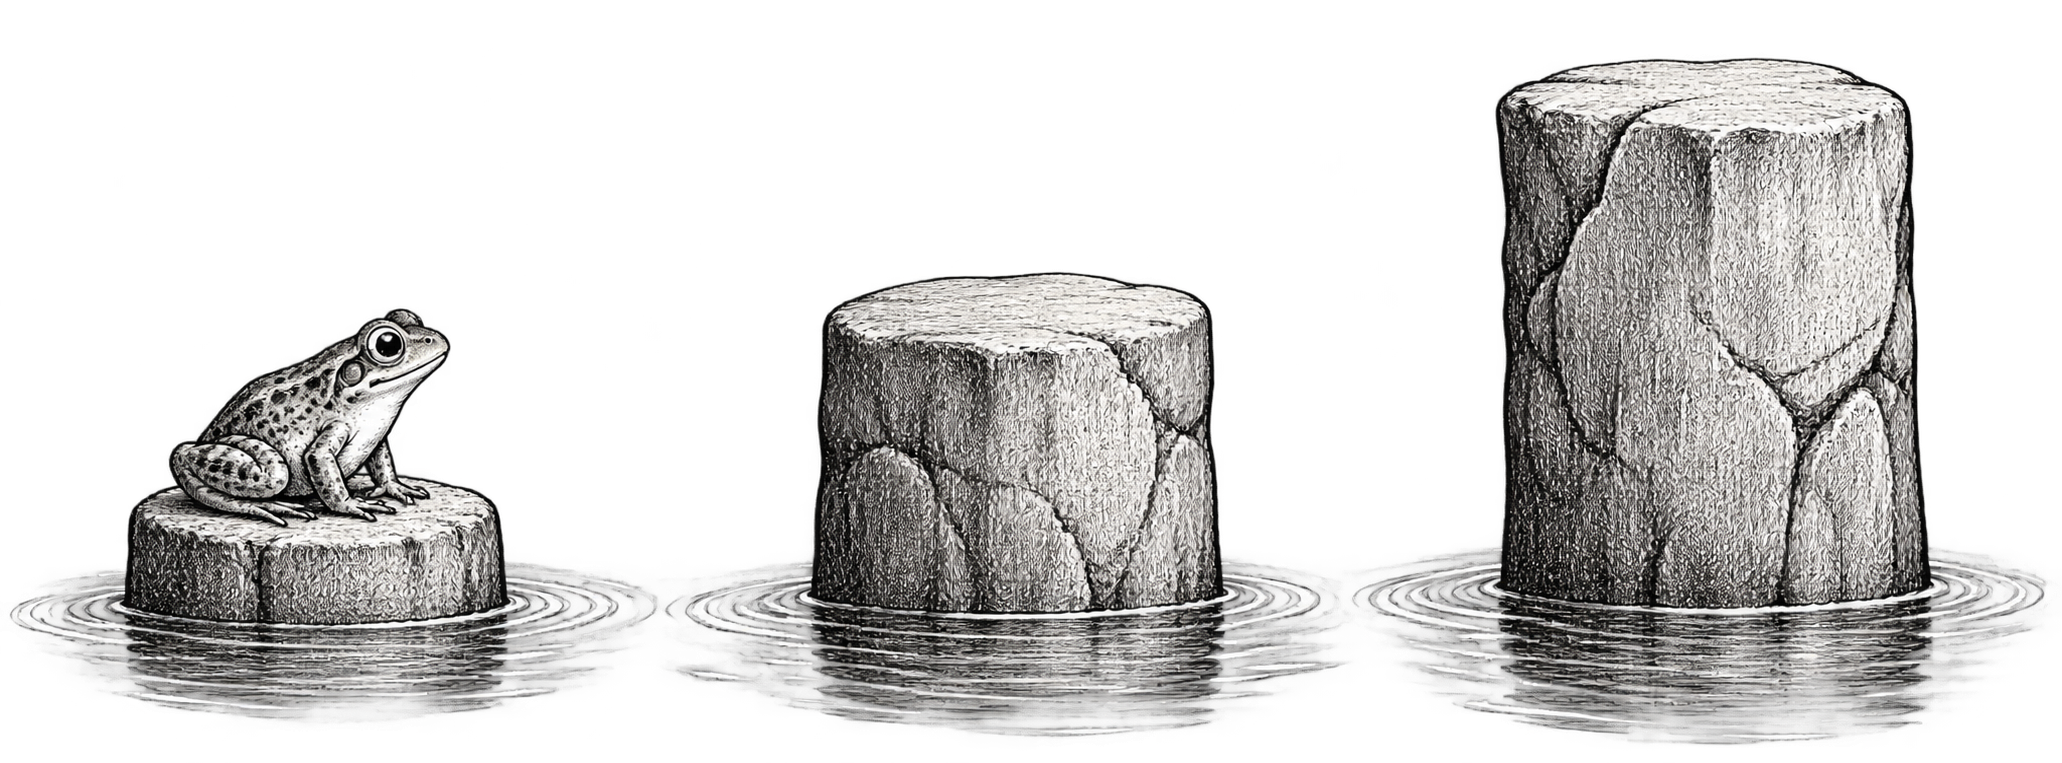
\includegraphics[width=18cm,height=3.6cm,keepaspectratio]{assets/slides/frog-stones.png}};
\node[anchor=north west,inner sep=0pt,text width=28cm,align=left,text=quiet,font=\fontsize{12}{\dimexpr12pt*6/5\relax}\selectfont] at (1.5,0.8) {Lesson 1 / FROG / OUR NEXT QUESTION};
\node[anchor=north west,inner sep=0pt,text width=1cm,align=left,text=quiet,font=\fontsize{11}{\dimexpr11pt*6/5\relax}\selectfont] at (30,0.8) {\insertframenumber};
\end{scope}\end{tikzpicture}
\end{frame}

\begin{frame}[plain,fragile]\begin{tikzpicture}[remember picture,overlay,x=1cm,y=1cm]\begin{scope}[shift={(current page.south west)}]
\node[anchor=north west,inner sep=0pt,text width=29cm,align=left,text=quiet,font=\fontsize{12}{\dimexpr12pt*6/5\relax}\selectfont] at (1.5,0.8) {Lesson 1 / FROG / L1-14 / QUESTION};
\node[anchor=north west,inner sep=0pt,text width=1cm,align=left,text=quiet,font=\fontsize{11}{\dimexpr11pt*6/5\relax}\selectfont] at (30,0.8) {\insertframenumber};
\node[anchor=north west,inner sep=0pt,text width=29cm,align=left,text=ink,font=\fontsize{40}{\dimexpr40pt*6/5\relax}\selectfont] at (1.5,16.5) {\heavy Frog: cost belongs to a whole route};
\node(body)[anchor=north west,inner sep=0pt,text width=29cm,align=left,text=ink,font=\fontsize{25}{\dimexpr25pt*6/5\relax}\selectfont] at (1.5,13.0) {Number the stones 0, 1 and 2; their heights are [10, 20, 30]. A frog starts at stone 0 and may jump forward one or two positions. A jump costs the absolute height difference, so a drop of 10 also costs 10. List all routes to stone 2 and add the jump costs for each.};
\node[anchor=south,inner sep=0] at (16,2.1) {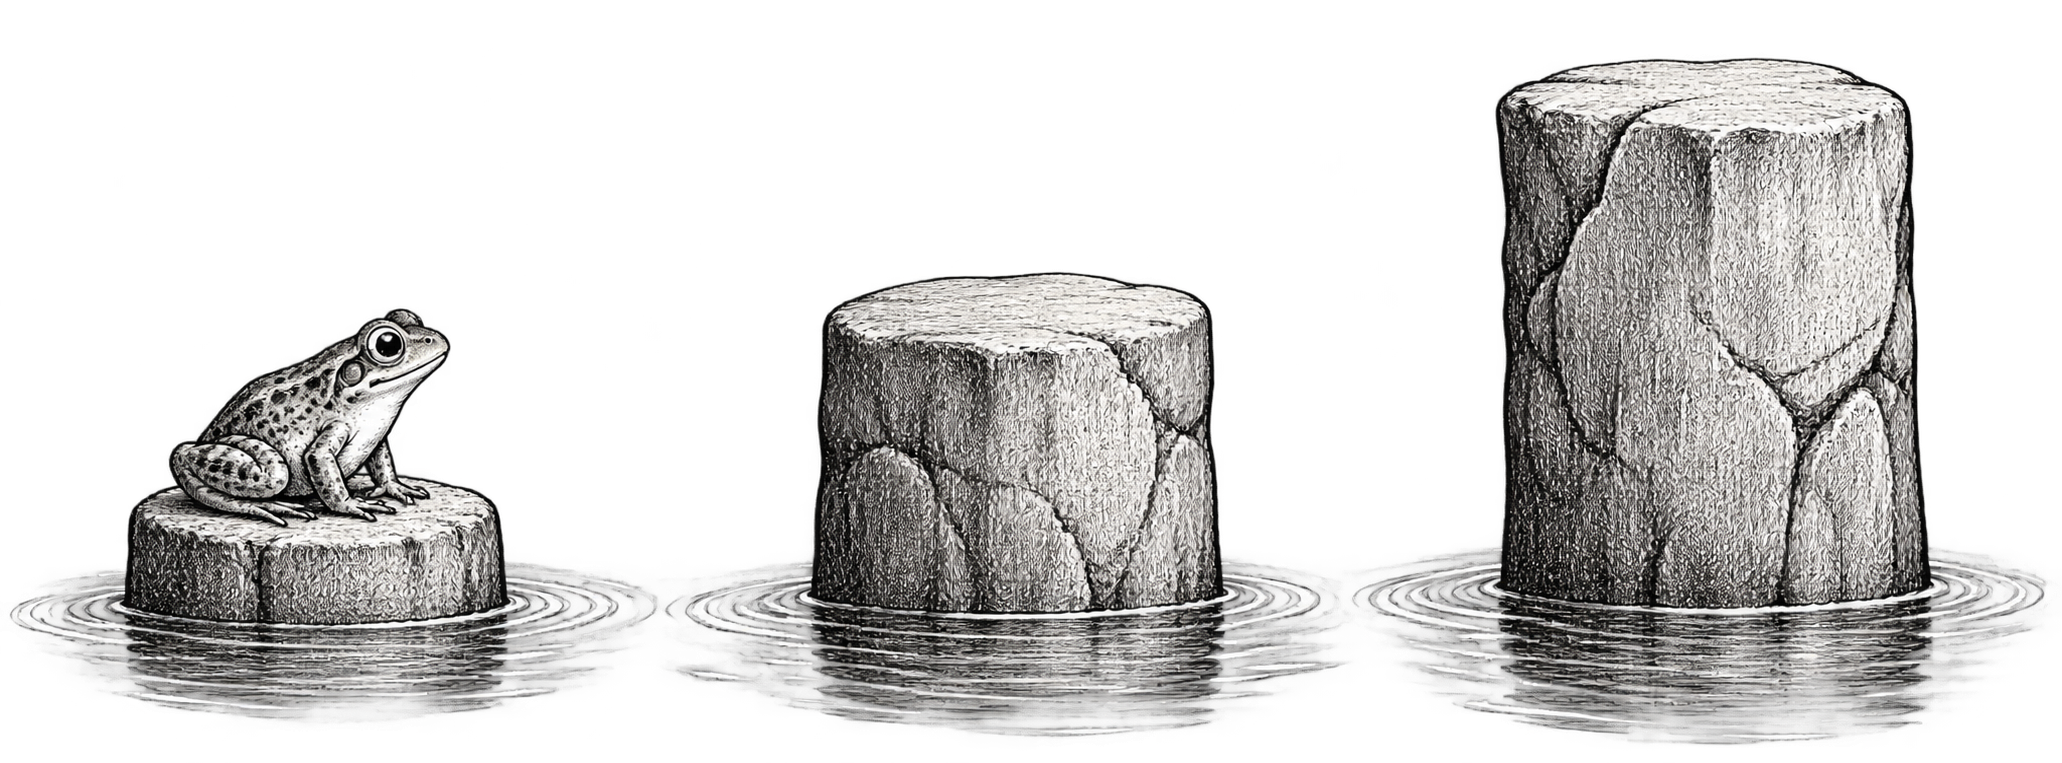
\includegraphics[width=24cm,height=5.7cm,keepaspectratio]{assets/slides/frog-stones.png}};
\node[anchor=north west,inner sep=0pt,text width=28cm,align=left,text=quiet,font=\fontsize{17}{\dimexpr17pt*6/5\relax}\selectfont] at (1.5,1.45) {Think on your own first. Then compare your reasoning with a partner.};
\end{scope}\end{tikzpicture}
\end{frame}

\begin{frame}[plain,fragile]
\begin{tikzpicture}[remember picture,overlay,x=1cm,y=1cm]\begin{scope}[shift={(current page.south west)}]
\node[anchor=north west,inner sep=0pt,text width=29cm,align=left,text=quiet,font=\fontsize{12}{\dimexpr12pt*6/5\relax}\selectfont] at (1.5,0.8) {Lesson 1 / FROG / L1-14 / ANSWER};
\node[anchor=north west,inner sep=0pt,text width=1cm,align=left,text=quiet,font=\fontsize{11}{\dimexpr11pt*6/5\relax}\selectfont] at (30,0.8) {\insertframenumber};
\node[anchor=north west,inner sep=0pt,text width=29cm,align=left,text=ink,font=\fontsize{40}{\dimexpr40pt*6/5\relax}\selectfont] at (1.5,16.5) {\heavy Frog: cost belongs to a whole route};
\node(body)[anchor=north west,inner sep=0pt,text width=29cm,align=left,text=ink,font=\fontsize{25}{\dimexpr25pt*6/5\relax}\selectfont] at (1.5,13.0) {The routes are 0, 1, 2 with cost 10 + 10 = 20, and 0, 2 with cost 20. Both are optimal. A cost is never negative: abs(10 - 30) = 20.};
\node[anchor=north west,inner sep=0pt,text width=28cm,align=left,text=quiet,font=\fontsize{21}{\dimexpr21pt*6/5\relax}\selectfont] at (1.5,4.0) {\textbf{Watch for:} Minimising the number of jumps is not the same as minimising height-difference cost.};
\end{scope}\end{tikzpicture}
\end{frame}

\begin{frame}[plain,fragile]\begin{tikzpicture}[remember picture,overlay,x=1cm,y=1cm]\begin{scope}[shift={(current page.south west)}]
\node[anchor=north west,inner sep=0pt,text width=29cm,align=left,text=quiet,font=\fontsize{12}{\dimexpr12pt*6/5\relax}\selectfont] at (1.5,0.8) {Lesson 1 / FROG / L1-15 / QUESTION};
\node[anchor=north west,inner sep=0pt,text width=1cm,align=left,text=quiet,font=\fontsize{11}{\dimexpr11pt*6/5\relax}\selectfont] at (30,0.8) {\insertframenumber};
\node[anchor=north west,inner sep=0pt,text width=29cm,align=left,text=ink,font=\fontsize{40}{\dimexpr40pt*6/5\relax}\selectfont] at (1.5,16.5) {\heavy A greedy choice can fail};
\node(body)[anchor=north west,inner sep=0pt,text width=29cm,align=left,text=ink,font=\fontsize{22}{\dimexpr22pt*6/5\relax}\selectfont] at (1.5,13.0) {Use heights [20, 50, 30, 40, 10, 10], at stones 0 through 5. At each stone, choose the cheaper of the next two legal jumps; if costs tie, choose the farther stone. Trace this greedy route and its total cost. Can another complete route cost less?};
\node(tab)[anchor=north west,inner sep=0,text width=29cm] at ([yshift=-8mm]body.south west) {\begingroup\fontsize{22}{26}\selectfont\setlength{\tabcolsep}{5pt}\setlength{\arrayrulewidth}{.5pt}\arrayrulecolor{quiet}\renewcommand{\arraystretch}{1}\begin{tabularx}{\linewidth}{|>{\raggedright\arraybackslash}p{52mm}|>{\centering\arraybackslash}X|>{\centering\arraybackslash}X|>{\centering\arraybackslash}X|>{\centering\arraybackslash}X|>{\centering\arraybackslash}X|>{\centering\arraybackslash}X|}\hline
\rowcolor{wash}\rule[-3mm]{0pt}{9.5mm}\textbf{Stone i} & \textbf{0} & \textbf{1} & \textbf{2} & \textbf{3} & \textbf{4} & \textbf{5}\\\hline
\rule[-4.6mm]{0pt}{13.5mm}heights[i] & 20 & 50 & 30 & 40 & 10 & 10\\\hline
\end{tabularx}\endgroup};
\end{scope}\end{tikzpicture}
\end{frame}

\begin{frame}[plain,fragile]\begin{tikzpicture}[remember picture,overlay,x=1cm,y=1cm]\begin{scope}[shift={(current page.south west)}]
\node[anchor=north west,inner sep=0pt,text width=29cm,align=left,text=quiet,font=\fontsize{12}{\dimexpr12pt*6/5\relax}\selectfont] at (1.5,0.8) {Lesson 1 / FROG / L1-15 / ANSWER};
\node[anchor=north west,inner sep=0pt,text width=1cm,align=left,text=quiet,font=\fontsize{11}{\dimexpr11pt*6/5\relax}\selectfont] at (30,0.8) {\insertframenumber};
\node[anchor=north west,inner sep=0pt,text width=29cm,align=left,text=ink,font=\fontsize{40}{\dimexpr40pt*6/5\relax}\selectfont] at (1.5,16.5) {\heavy A greedy choice can fail};
\node(body)[anchor=north west,inner sep=0pt,text width=29cm,align=left,text=ink,font=\fontsize{22}{\dimexpr22pt*6/5\relax}\selectfont] at (1.5,13.0) {Greedy can take stones 0, 2, 3, 5: cost 10 + 10 + 30 = 50. The optimal route 0, 2, 4, 5 costs 10 + 20 + 0 = 30. Paying more at stone 2 saves cost later.};
\node(tab)[anchor=north west,inner sep=0,text width=29cm] at ([yshift=-8mm]body.south west) {\begingroup\fontsize{22}{26}\selectfont\setlength{\tabcolsep}{5pt}\setlength{\arrayrulewidth}{.5pt}\arrayrulecolor{quiet}\renewcommand{\arraystretch}{1}\begin{tabularx}{\linewidth}{|>{\raggedright\arraybackslash}p{88mm}|>{\centering\arraybackslash}X|>{\centering\arraybackslash}X|>{\centering\arraybackslash}X|>{\centering\arraybackslash}X|>{\centering\arraybackslash}X|>{\centering\arraybackslash}X|>{\centering\arraybackslash}X|}\hline
\rowcolor{wash}\rule[-3mm]{0pt}{9.5mm}\textbf{Jump into stone i} & \textbf{0} & \textbf{1} & \textbf{2} & \textbf{3} & \textbf{4} & \textbf{5} & \textbf{Total}\\\hline
\rule[-4.6mm]{0pt}{13.5mm}heights[i] & 20 & 50 & 30 & 40 & 10 & 10 & \\\hline
\rule[-4.6mm]{0pt}{13.5mm}greedy 0, 2, 3, 5 & start &  & 10 & 10 &  & 30 & 50\\\hline
\rule[-4.6mm]{0pt}{13.5mm}best 0, 2, 4, 5 & start &  & 10 &  & 20 & 0 & 30\\\hline
\end{tabularx}\endgroup};
\end{scope}\end{tikzpicture}
\end{frame}

\begin{frame}[plain,fragile]\begin{tikzpicture}[remember picture,overlay,x=1cm,y=1cm]\begin{scope}[shift={(current page.south west)}]
\node[anchor=north west,inner sep=0pt,text width=29cm,align=left,text=quiet,font=\fontsize{12}{\dimexpr12pt*6/5\relax}\selectfont] at (1.5,0.8) {Lesson 1 / FROG / L1-16 / GRAPH / QUESTION};
\node[anchor=north west,inner sep=0pt,text width=1cm,align=left,text=quiet,font=\fontsize{11}{\dimexpr11pt*6/5\relax}\selectfont] at (30,0.8) {\insertframenumber};
\node[anchor=north west,inner sep=0pt,text width=29cm,align=left,text=ink,font=\fontsize{40}{\dimexpr40pt*6/5\relax}\selectfont] at (1.5,16.5) {\heavy The same connections as the stairs};
\node[anchor=north west,inner sep=0pt,text width=29cm,align=left,text=ink,font=\fontsize{20}{\dimexpr20pt*6/5\relax}\selectfont] at (1.5,13.4) {Data: heights [20, 50, 30, 40, 10, 10]. Stone indices run from 0 to 5.};
\node[anchor=north west,inner sep=0] at (3,11.8) {\resizebox{25cm}{!}{\begin{tikzpicture}[x=1cm,y=1cm,>=Stealth,every node/.style={font=\small}]
\node[draw=ink,circle,minimum size=8mm,fill=codepaper] (g0) at (0,0) {0};
\node[below=3mm] at (g0.south) {height 20};
\node[draw=ink,circle,minimum size=8mm,fill=codepaper] (g1) at (2,0) {1};
\node[below=3mm] at (g1.south) {height 50};
\node[draw=ink,circle,minimum size=8mm,fill=codepaper] (g2) at (4,0) {2};
\node[below=3mm] at (g2.south) {height 30};
\node[draw=ink,circle,minimum size=8mm,fill=codepaper] (g3) at (6,0) {3};
\node[below=3mm] at (g3.south) {height 40};
\node[draw=ink,circle,minimum size=8mm,fill=codepaper] (g4) at (8,0) {4};
\node[below=3mm] at (g4.south) {height 10};
\node[draw=ink,circle,minimum size=8mm,fill=codepaper] (g5) at (10,0) {5};
\node[below=3mm] at (g5.south) {height 10};
\draw[->,draw=ink] (g0.east) -- node[above,fill=white,inner sep=2pt] {30} (g1.west);
\draw[->,draw=ink] (g0.north) to[bend left=45] node[above,fill=white,inner sep=2pt] {10} (g2.north);
\draw[->,draw=ink] (g1.east) -- node[above,fill=white,inner sep=2pt] {20} (g2.west);
\draw[->,draw=ink] (g1.north) to[bend left=45] node[above,fill=white,inner sep=2pt] {10} (g3.north);
\draw[->,draw=ink] (g2.east) -- node[above,fill=white,inner sep=2pt] {10} (g3.west);
\draw[->,draw=ink] (g2.north) to[bend left=45] node[above,fill=white,inner sep=2pt] {20} (g4.north);
\draw[->,draw=ink] (g3.east) -- node[above,fill=white,inner sep=2pt] {30} (g4.west);
\draw[->,draw=ink] (g3.north) to[bend left=45] node[above,fill=white,inner sep=2pt] {30} (g5.north);
\draw[->,draw=ink] (g4.east) -- node[above,fill=white,inner sep=2pt] {0} (g5.west);
\end{tikzpicture}}};
\node[anchor=north west,inner sep=0pt,text width=29cm,align=left,text=ink,font=\fontsize{21}{\dimexpr21pt*6/5\relax}\selectfont] at (1.5,5.6) {Circles show stone indices; arrows show legal jumps and their costs.

Which arrows enter stone 4? What must we know before choosing the cheapest route into it?};
\end{scope}\end{tikzpicture}
\end{frame}

\begin{frame}[plain,fragile]\begin{tikzpicture}[remember picture,overlay,x=1cm,y=1cm]\begin{scope}[shift={(current page.south west)}]
\node[anchor=north west,inner sep=0pt,text width=29cm,align=left,text=quiet,font=\fontsize{12}{\dimexpr12pt*6/5\relax}\selectfont] at (1.5,0.8) {Lesson 1 / FROG / L1-16 / GRAPH / ANSWER};
\node[anchor=north west,inner sep=0pt,text width=1cm,align=left,text=quiet,font=\fontsize{11}{\dimexpr11pt*6/5\relax}\selectfont] at (30,0.8) {\insertframenumber};
\node[anchor=north west,inner sep=0pt,text width=29cm,align=left,text=ink,font=\fontsize{40}{\dimexpr40pt*6/5\relax}\selectfont] at (1.5,16.5) {\heavy Compare complete costs into a stone};
\node[anchor=north west,inner sep=0pt,text width=29cm,align=left,text=ink,font=\fontsize{20}{\dimexpr20pt*6/5\relax}\selectfont] at (1.5,13.4) {Data: heights [20, 50, 30, 40, 10, 10]. Stone indices run from 0 to 5.};
\node[anchor=north west,inner sep=0] at (3,11.8) {\resizebox{25cm}{!}{\begin{tikzpicture}[x=1cm,y=1cm,>=Stealth,every node/.style={font=\small}]
\node[draw=ink,circle,minimum size=8mm,fill=codepaper] (g0) at (0,0) {0};
\node[below=3mm] at (g0.south) {height 20};
\node[draw=ink,circle,minimum size=8mm,fill=codepaper] (g1) at (2,0) {1};
\node[below=3mm] at (g1.south) {height 50};
\node[draw=ink,circle,minimum size=8mm,fill=codepaper] (g2) at (4,0) {2};
\node[below=3mm] at (g2.south) {height 30};
\node[draw=ink,circle,minimum size=8mm,fill=codepaper] (g3) at (6,0) {3};
\node[below=3mm] at (g3.south) {height 40};
\node[draw=ink,circle,minimum size=8mm,fill=codepaper] (g4) at (8,0) {4};
\node[below=3mm] at (g4.south) {height 10};
\node[draw=ink,circle,minimum size=8mm,fill=codepaper] (g5) at (10,0) {5};
\node[below=3mm] at (g5.south) {height 10};
\draw[->,draw=ink] (g0.east) -- node[above,fill=white,inner sep=2pt] {30} (g1.west);
\draw[->,draw=ink] (g0.north) to[bend left=45] node[above,fill=white,inner sep=2pt] {10} (g2.north);
\draw[->,draw=ink] (g1.east) -- node[above,fill=white,inner sep=2pt] {20} (g2.west);
\draw[->,draw=ink] (g1.north) to[bend left=45] node[above,fill=white,inner sep=2pt] {10} (g3.north);
\draw[->,draw=ink] (g2.east) -- node[above,fill=white,inner sep=2pt] {10} (g3.west);
\draw[->,draw=ink] (g2.north) to[bend left=45] node[above,fill=white,inner sep=2pt] {20} (g4.north);
\draw[->,draw=ink] (g3.east) -- node[above,fill=white,inner sep=2pt] {30} (g4.west);
\draw[->,draw=ink] (g3.north) to[bend left=45] node[above,fill=white,inner sep=2pt] {30} (g5.north);
\draw[->,draw=ink] (g4.east) -- node[above,fill=white,inner sep=2pt] {0} (g5.west);
\end{tikzpicture}}};
\node[anchor=north west,inner sep=0pt,text width=29cm,align=left,text=ink,font=\fontsize{21}{\dimexpr21pt*6/5\relax}\selectfont] at (1.5,5.6) {Suppose the cheapest costs to stones 3 and 2 are already known: 20 and 10. To stone 4 via stone 3: 20 + 30 = 50. Via stone 2: 10 + 20 = 30. Choose 30.

Stairs adds route counts. Frog takes the smaller total cost. One graph node represents a stone; the recursion tree may ask for that stone repeatedly.};
\end{scope}\end{tikzpicture}
\end{frame}

\begin{frame}[plain,fragile]\begin{tikzpicture}[remember picture,overlay,x=1cm,y=1cm]\begin{scope}[shift={(current page.south west)}]
\node[anchor=north west,inner sep=0pt,text width=29cm,align=left,text=quiet,font=\fontsize{12}{\dimexpr12pt*6/5\relax}\selectfont] at (1.5,0.8) {Lesson 1 / FROG / L1-16 / QUESTION};
\node[anchor=north west,inner sep=0pt,text width=1cm,align=left,text=quiet,font=\fontsize{11}{\dimexpr11pt*6/5\relax}\selectfont] at (30,0.8) {\insertframenumber};
\node[anchor=north west,inner sep=0pt,text width=29cm,align=left,text=ink,font=\fontsize{40}{\dimexpr40pt*6/5\relax}\selectfont] at (1.5,16.5) {\heavy Frog: ask about the last jump};
\node(body)[anchor=north west,inner sep=0pt,text width=29cm,align=left,text=ink,font=\fontsize{20}{\dimexpr20pt*6/5\relax}\selectfont] at (1.5,13.0) {Write frog\_slow(heights) with recursive helper cost(i): the cheapest total cost from stone 0 to stone i. Which earlier stones can supply the last jump? Explore both possibilities.};
\node(sig)[anchor=north west,inner sep=3mm,fill=codepaper,align=left,font=\ttfamily\fontsize{16}{20}\selectfont] at ([yshift=-4mm,xshift=3mm]body.south west) {def frog\_slow(heights):\\\hspace*{2.4em}def cost(i):\\\hspace*{4.8em}return None  \# Replace this\\\hspace*{2.4em}return cost(len(heights) - 1)};
\node(result)[anchor=north west,inner sep=0pt,text width=13.5cm,align=left,text=quiet,font=\fontsize{17}{20}\selectfont] at ([yshift=-4mm,xshift=15.5cm]body.south west) {\textbf{Returns}\par \textbf{frog\_slow(heights)}: the cheapest total cost from stone 0 to the last stone.\par\smallskip \textbf{cost(i)}: the cheapest total cost from stone 0 to stone i, including all jumps along the route.\par\smallskip };
\node(both)[fit=(sig)(result),inner sep=0] {};
\node[anchor=north west,inner sep=0pt,text width=29cm,align=left,text=quiet,font=\fontsize{18}{22}\selectfont] at ([yshift=-3mm,xshift=-3mm]both.south west) {\textbf{Hints.} What is the smallest i you can answer directly? Which earlier stones can the last jump into stone i start from? What does cost(i) need to know about each of those stones?};
\end{scope}\end{tikzpicture}
\end{frame}

\begin{frame}[plain,fragile]\begin{tikzpicture}[remember picture,overlay,x=1cm,y=1cm]\begin{scope}[shift={(current page.south west)}]
\node[anchor=north west,inner sep=0pt,text width=29cm,align=left,text=quiet,font=\fontsize{12}{\dimexpr12pt*6/5\relax}\selectfont] at (1.5,0.8) {Lesson 1 / FROG / L1-16 / ANSWER};
\node[anchor=north west,inner sep=0pt,text width=1cm,align=left,text=quiet,font=\fontsize{11}{\dimexpr11pt*6/5\relax}\selectfont] at (30,0.8) {\insertframenumber};
\node[anchor=north west,inner sep=0pt,text width=29cm,align=left,text=ink,font=\fontsize{40}{\dimexpr40pt*6/5\relax}\selectfont] at (1.5,16.5) {\heavy Frog: ask about the last jump};
\node(body)[anchor=north west,inner sep=0pt,text width=29cm,align=left,text=ink,font=\fontsize{20}{\dimexpr20pt*6/5\relax}\selectfont] at (1.5,13.0) {Try i - 1 and, when it exists, i - 2. Add the last jump cost to the cheapest cost of reaching that earlier stone, then take the minimum. cost(0) is 0 because the frog starts there.};
\node[anchor=north west,inner sep=0pt,text width=29cm,align=left,text=quiet,font=\fontsize{18}{\dimexpr18pt*6/5\relax}\selectfont] at (1.5,9.6) {Data: heights = [20, 50, 30, 40, 10, 10]. Arrows label the final jump cost.};
\node(a)[draw=callink,line width=1.3pt,fill=callwash,rounded corners=3mm,minimum width=5.1cm,minimum height=1.15cm,align=center,font=\fontsize{18}{22}\selectfont] at (16,8.3) {cost(5) = 30};
\node(b)[draw=callink,line width=1.3pt,fill=callwash,rounded corners=3mm,minimum width=5.1cm,minimum height=1.15cm,align=center,font=\fontsize{18}{22}\selectfont] at (9,5.9) {cost(4) = 30};
\node(c)[draw=waitink,line width=1.3pt,fill=waitwash,rounded corners=3mm,minimum width=5.1cm,minimum height=1.15cm,align=center,font=\fontsize{18}{22}\selectfont] at (24,5.9) {cost(3) = 20};
\node(d)[draw=waitink,line width=1.3pt,fill=waitwash,rounded corners=3mm,minimum width=5.1cm,minimum height=1.15cm,align=center,font=\fontsize{18}{22}\selectfont] at (3.8,3.5) {cost(3) = 20};
\node(e)[draw=waitink,line width=1.3pt,fill=waitwash,rounded corners=3mm,minimum width=5.1cm,minimum height=1.15cm,align=center,font=\fontsize{18}{22}\selectfont] at (12,3.5) {cost(2) = 10};
\node(f)[draw=waitink,line width=1.3pt,fill=waitwash,rounded corners=3mm,minimum width=5.1cm,minimum height=1.15cm,align=center,font=\fontsize{18}{22}\selectfont] at (21,3.5) {cost(2) = 10};
\node(g)[draw=callink,line width=1.3pt,fill=callwash,rounded corners=3mm,minimum width=5.1cm,minimum height=1.15cm,align=center,font=\fontsize{18}{22}\selectfont] at (28,3.5) {cost(1) = 30};
\draw[-{Stealth[length=3mm]},line width=1.5pt,callink] (a.south)--node[midway,fill=white,inner sep=2pt,font=\fontsize{15}{18}\selectfont,text=callink]{+0}(b.north);
\draw[-{Stealth[length=3mm]},line width=1.5pt,callink] (a.south)--node[midway,fill=white,inner sep=2pt,font=\fontsize{15}{18}\selectfont,text=callink]{+30}(c.north);
\draw[-{Stealth[length=3mm]},line width=1.5pt,callink] (b.south)--node[midway,fill=white,inner sep=2pt,font=\fontsize{15}{18}\selectfont,text=callink]{+30}(d.north);
\draw[-{Stealth[length=3mm]},line width=1.5pt,callink] (b.south)--node[midway,fill=white,inner sep=2pt,font=\fontsize{15}{18}\selectfont,text=callink]{+20}(e.north);
\draw[-{Stealth[length=3mm]},line width=1.5pt,callink] (c.south)--node[midway,fill=white,inner sep=2pt,font=\fontsize{15}{18}\selectfont,text=callink]{+10}(f.north);
\draw[-{Stealth[length=3mm]},line width=1.5pt,callink] (c.south)--node[midway,fill=white,inner sep=2pt,font=\fontsize{15}{18}\selectfont,text=callink]{+10}(g.north);
\node[anchor=north west,inner sep=0pt,text width=29cm,align=left,text=quiet,font=\fontsize{19}{\dimexpr19pt*6/5\relax}\selectfont] at (1.5,1.7) {At stone 5: min(30 + 0, 20 + 30) = 30. Only the first three call levels are shown.};
\end{scope}\end{tikzpicture}
\end{frame}

\begin{frame}[plain,fragile]
\begin{lrbox}{\codebox}\begin{minipage}{792pt}
\begin{lstlisting}[basicstyle=\ttfamily\fontsize{21.0}{23.5}\selectfont\color{ink},numbers=left,numberstyle=\ttfamily\fontsize{13.7}{23.5}\selectfont\color{quiet},numbersep=12pt,xleftmargin=30pt,firstnumber=1,breaklines=false,aboveskip=0pt,belowskip=0pt]
def frog_slow(heights):
    def cost(i):
        if i == 0:
            return 0
        one = cost(i - 1) + abs(heights[i] - heights[i - 1])
        if i == 1:
            return one
        two = cost(i - 2) + abs(heights[i] - heights[i - 2])
        return min(one, two)
    return cost(len(heights) - 1)
\end{lstlisting}
\end{minipage}\end{lrbox}
\begin{tikzpicture}[remember picture,overlay,x=1cm,y=1cm]\begin{scope}[shift={(current page.south west)}]
\node[anchor=north west,inner sep=0pt,text width=29cm,align=left,text=quiet,font=\fontsize{12}{\dimexpr12pt*6/5\relax}\selectfont] at (1.5,0.8) {Lesson 1 / FROG / L1-16 / ANSWER: PYTHON};
\node[anchor=north west,inner sep=0pt,text width=1cm,align=left,text=quiet,font=\fontsize{11}{\dimexpr11pt*6/5\relax}\selectfont] at (30,0.8) {\insertframenumber};
\node[anchor=north west,inner sep=0pt,text width=29cm,align=left,text=ink,font=\fontsize{40}{48}\selectfont] at (1.5,16.5) {\heavy frog\_slow(heights)};
\node[anchor=north,inner sep=5mm,fill=codepaper] at (16,13.0) {\usebox{\codebox}};
\end{scope}\end{tikzpicture}

\end{frame}

\begin{frame}[plain,fragile]\begin{tikzpicture}[remember picture,overlay,x=1cm,y=1cm]\begin{scope}[shift={(current page.south west)}]
\node[anchor=north west,inner sep=0pt,text width=29cm,align=left,text=quiet,font=\fontsize{12}{\dimexpr12pt*6/5\relax}\selectfont] at (1.5,0.8) {Lesson 1 / FROG / L1-17 / QUESTION};
\node[anchor=north west,inner sep=0pt,text width=1cm,align=left,text=quiet,font=\fontsize{11}{\dimexpr11pt*6/5\relax}\selectfont] at (30,0.8) {\insertframenumber};
\node[anchor=north west,inner sep=0pt,text width=29cm,align=left,text=ink,font=\fontsize{40}{\dimexpr40pt*6/5\relax}\selectfont] at (1.5,16.5) {\heavy Frog: cache the stone number};
\node(body)[anchor=north west,inner sep=0pt,text width=29cm,align=left,text=ink,font=\fontsize{25}{\dimexpr25pt*6/5\relax}\selectfont] at (1.5,13.0) {In the recursive Frog solution, what is the cache key? Why can different routes that reach the same stone share an answer?};
\node[anchor=north west,inner sep=0pt,text width=28cm,align=left,text=quiet,font=\fontsize{22}{\dimexpr22pt*6/5\relax}\selectfont] at (1.5,4.0) {Think on your own first. Then compare your reasoning with a partner.};
\end{scope}\end{tikzpicture}
\end{frame}

\begin{frame}[plain,fragile]\begin{tikzpicture}[remember picture,overlay,x=1cm,y=1cm]\begin{scope}[shift={(current page.south west)}]
\node[anchor=north west,inner sep=0pt,text width=29cm,align=left,text=quiet,font=\fontsize{12}{\dimexpr12pt*6/5\relax}\selectfont] at (1.5,0.8) {Lesson 1 / FROG / L1-17 / ANSWER};
\node[anchor=north west,inner sep=0pt,text width=1cm,align=left,text=quiet,font=\fontsize{11}{\dimexpr11pt*6/5\relax}\selectfont] at (30,0.8) {\insertframenumber};
\node[anchor=north west,inner sep=0pt,text width=29cm,align=left,text=ink,font=\fontsize{40}{\dimexpr40pt*6/5\relax}\selectfont] at (1.5,16.5) {\heavy Frog: cache the stone number};
\node(body)[anchor=north west,inner sep=0pt,text width=29cm,align=left,text=ink,font=\fontsize{25}{\dimexpr25pt*6/5\relax}\selectfont] at (1.5,13.0) {The key is the stone index i. cost(i) always asks for the cheapest cost from the fixed start to that stone. The fixed height list and allowed jumps are the same in every call, so one answer per i is enough.};
\node[anchor=north west,inner sep=0pt,text width=28cm,align=left,text=quiet,font=\fontsize{21}{\dimexpr21pt*6/5\relax}\selectfont] at (1.5,4.0) {\textbf{Watch for:} A global cache keyed only by i becomes stale if you change the height list.};
\end{scope}\end{tikzpicture}
\end{frame}

\begin{frame}[plain,fragile]
\begin{lrbox}{\codebox}\begin{minipage}{789pt}
\begin{lstlisting}[basicstyle=\ttfamily\fontsize{18.5}{20.7}\selectfont\color{ink},numbers=left,numberstyle=\ttfamily\fontsize{12.0}{20.7}\selectfont\color{quiet},numbersep=12pt,xleftmargin=28pt,firstnumber=1,breaklines=false,aboveskip=0pt,belowskip=0pt]
def frog_cached(heights):
    cache = {0: 0}
    def cost(i):
        if i not in cache:
            one = cost(i - 1) + abs(heights[i] - heights[i - 1])
            answer = one
            if i >= 2:
                two = cost(i - 2) + abs(heights[i] - heights[i - 2])
                answer = min(one, two)
            cache[i] = answer
        return cache[i]
    return cost(len(heights) - 1)
\end{lstlisting}
\end{minipage}\end{lrbox}
\begin{tikzpicture}[remember picture,overlay,x=1cm,y=1cm]\begin{scope}[shift={(current page.south west)}]
\node[anchor=north west,inner sep=0pt,text width=29cm,align=left,text=quiet,font=\fontsize{12}{\dimexpr12pt*6/5\relax}\selectfont] at (1.5,0.8) {Lesson 1 / FROG / L1-17 / ANSWER: PYTHON};
\node[anchor=north west,inner sep=0pt,text width=1cm,align=left,text=quiet,font=\fontsize{11}{\dimexpr11pt*6/5\relax}\selectfont] at (30,0.8) {\insertframenumber};
\node[anchor=north west,inner sep=0pt,text width=29cm,align=left,text=ink,font=\fontsize{40}{48}\selectfont] at (1.5,16.5) {\heavy frog\_cached(heights)};
\node[anchor=north,inner sep=5mm,fill=codepaper] at (16,13.0) {\usebox{\codebox}};
\end{scope}\end{tikzpicture}

\end{frame}

\begin{frame}[plain,fragile]\begin{tikzpicture}[remember picture,overlay,x=1cm,y=1cm]\begin{scope}[shift={(current page.south west)}]
\node[anchor=north west,inner sep=0pt,text width=29cm,align=left,text=quiet,font=\fontsize{12}{\dimexpr12pt*6/5\relax}\selectfont] at (1.5,0.8) {Lesson 1 / FROG / L1-18 / QUESTION};
\node[anchor=north west,inner sep=0pt,text width=1cm,align=left,text=quiet,font=\fontsize{11}{\dimexpr11pt*6/5\relax}\selectfont] at (30,0.8) {\insertframenumber};
\node[anchor=north west,inner sep=0pt,text width=29cm,align=left,text=ink,font=\fontsize{40}{\dimexpr40pt*6/5\relax}\selectfont] at (1.5,16.5) {\heavy Frog: write the iterative solution};
\node(body)[anchor=north west,inner sep=0pt,text width=29cm,align=left,text=ink,font=\fontsize{20}{\dimexpr20pt*6/5\relax}\selectfont] at (1.5,13.0) {Write frog\_table(heights) using a loop. Return the cheapest total cost from stone 0 to the last stone. First fill best[i] for heights [20, 50, 30, 40, 10, 10], then turn those steps into Python code. Explain why the loop runs from left to right. Test your function on these heights.};
\node(tab)[anchor=north west,inner sep=0,text width=29cm] at ([yshift=-8mm]body.south west) {\begingroup\fontsize{18}{22}\selectfont\setlength{\tabcolsep}{5pt}\setlength{\arrayrulewidth}{.5pt}\arrayrulecolor{quiet}\renewcommand{\arraystretch}{1}\begin{tabularx}{\linewidth}{|>{\raggedright\arraybackslash}p{52mm}|>{\centering\arraybackslash}X|>{\centering\arraybackslash}X|>{\centering\arraybackslash}X|>{\centering\arraybackslash}X|>{\centering\arraybackslash}X|>{\centering\arraybackslash}X|}\hline
\rowcolor{wash}\rule[-2.6mm]{0pt}{8mm}\textbf{Stone i} & \textbf{0} & \textbf{1} & \textbf{2} & \textbf{3} & \textbf{4} & \textbf{5}\\\hline
\rule[-3.4mm]{0pt}{8.5mm}heights[i] & 20 & 50 & 30 & 40 & 10 & 10\\\hline
\rule[-3.4mm]{0pt}{8.5mm}best[i] & 0 &  &  &  &  & \\\hline
\end{tabularx}\endgroup};
\node(sig)[anchor=north west,inner sep=3mm,fill=codepaper,align=left,font=\ttfamily\fontsize{16}{20}\selectfont] at ([yshift=-4mm,xshift=3mm]tab.south west) {def frog\_table(heights):\\\hspace*{2.4em}return None  \# Replace this};
\node(result)[anchor=north west,inner sep=0pt,text width=13.5cm,align=left,text=quiet,font=\fontsize{17}{20}\selectfont] at ([yshift=-4mm,xshift=15.5cm]tab.south west) {\textbf{Returns}\par \textbf{frog\_table(heights)}: the cheapest total cost from stone 0 to the last stone.\par\smallskip };
\node(both)[fit=(sig)(result),inner sep=0] {};
\node[anchor=north west,inner sep=0pt,text width=29cm,align=left,text=quiet,font=\fontsize{18}{22}\selectfont] at ([yshift=-3mm,xshift=-3mm]both.south west) {\textbf{Hints.} What is best[0], before any jump? Which earlier entries does best[i] need, and are they filled when the loop reaches i?};
\end{scope}\end{tikzpicture}
\end{frame}

\begin{frame}[plain,fragile]\begin{tikzpicture}[remember picture,overlay,x=1cm,y=1cm]\begin{scope}[shift={(current page.south west)}]
\node[anchor=north west,inner sep=0pt,text width=29cm,align=left,text=quiet,font=\fontsize{12}{\dimexpr12pt*6/5\relax}\selectfont] at (1.5,0.8) {Lesson 1 / FROG / L1-18 / ANSWER};
\node[anchor=north west,inner sep=0pt,text width=1cm,align=left,text=quiet,font=\fontsize{11}{\dimexpr11pt*6/5\relax}\selectfont] at (30,0.8) {\insertframenumber};
\node[anchor=north west,inner sep=0pt,text width=29cm,align=left,text=ink,font=\fontsize{40}{\dimexpr40pt*6/5\relax}\selectfont] at (1.5,16.5) {\heavy Frog: write the iterative solution};
\node(body)[anchor=north west,inner sep=0pt,text width=29cm,align=left,text=ink,font=\fontsize{22}{\dimexpr22pt*6/5\relax}\selectfont] at (1.5,13.0) {The costs are [0, 30, 10, 20, 30, 30]. For stone 4, the two totals are 20 + 30 = 50 and 10 + 20 = 30. Every dependency has a smaller index, so it is already computed.};
\node(tab)[anchor=north west,inner sep=0,text width=29cm] at ([yshift=-8mm]body.south west) {\begingroup\fontsize{22}{26}\selectfont\setlength{\tabcolsep}{5pt}\setlength{\arrayrulewidth}{.5pt}\arrayrulecolor{quiet}\renewcommand{\arraystretch}{1}\begin{tabularx}{\linewidth}{|>{\raggedright\arraybackslash}p{52mm}|>{\centering\arraybackslash}X|>{\centering\arraybackslash}X|>{\centering\arraybackslash}X|>{\centering\arraybackslash}X|>{\centering\arraybackslash}X|>{\centering\arraybackslash}X|}\hline
\rowcolor{wash}\rule[-3mm]{0pt}{9.5mm}\textbf{Stone i} & \textbf{0} & \textbf{1} & \textbf{2} & \textbf{3} & \textbf{4} & \textbf{5}\\\hline
\rule[-4.6mm]{0pt}{13.5mm}heights[i] & 20 & 50 & 30 & 40 & 10 & 10\\\hline
\rule[-4.6mm]{0pt}{13.5mm}best[i] & 0 & 30 & 10 & 20 & 30 & 30\\\hline
\end{tabularx}\endgroup};
\end{scope}\end{tikzpicture}
\end{frame}

\begin{frame}[plain,fragile]
\begin{lrbox}{\codebox}\begin{minipage}{796pt}
\begin{lstlisting}[basicstyle=\ttfamily\fontsize{20.0}{22.4}\selectfont\color{ink},numbers=left,numberstyle=\ttfamily\fontsize{13.0}{22.4}\selectfont\color{quiet},numbersep=12pt,xleftmargin=22pt,firstnumber=1,breaklines=false,aboveskip=0pt,belowskip=0pt]
def frog_table(heights):
    best = [0] * len(heights)
    for i in range(1, len(heights)):
        best[i] = best[i - 1] + abs(heights[i] - heights[i - 1])
        if i >= 2:
            two = best[i - 2] + abs(heights[i] - heights[i - 2])
            best[i] = min(best[i], two)
    return best[-1]
\end{lstlisting}
\end{minipage}\end{lrbox}
\begin{tikzpicture}[remember picture,overlay,x=1cm,y=1cm]\begin{scope}[shift={(current page.south west)}]
\node[anchor=north west,inner sep=0pt,text width=29cm,align=left,text=quiet,font=\fontsize{12}{\dimexpr12pt*6/5\relax}\selectfont] at (1.5,0.8) {Lesson 1 / FROG / L1-18 / ANSWER: PYTHON};
\node[anchor=north west,inner sep=0pt,text width=1cm,align=left,text=quiet,font=\fontsize{11}{\dimexpr11pt*6/5\relax}\selectfont] at (30,0.8) {\insertframenumber};
\node[anchor=north west,inner sep=0pt,text width=29cm,align=left,text=ink,font=\fontsize{40}{48}\selectfont] at (1.5,16.5) {\heavy frog\_table(heights)};
\node[anchor=north,inner sep=5mm,fill=codepaper] at (16,13.0) {\usebox{\codebox}};
\end{scope}\end{tikzpicture}

\end{frame}

\begin{frame}[plain,fragile]\begin{tikzpicture}[remember picture,overlay,x=1cm,y=1cm]\begin{scope}[shift={(current page.south west)}]
\node[anchor=north west,inner sep=0pt,text width=29cm,align=left,text=quiet,font=\fontsize{12}{\dimexpr12pt*6/5\relax}\selectfont] at (1.5,0.8) {Lesson 1 / FROG / L1-19 / QUESTION};
\node[anchor=north west,inner sep=0pt,text width=1cm,align=left,text=quiet,font=\fontsize{11}{\dimexpr11pt*6/5\relax}\selectfont] at (30,0.8) {\insertframenumber};
\node[anchor=north west,inner sep=0pt,text width=29cm,align=left,text=ink,font=\fontsize{40}{\dimexpr40pt*6/5\relax}\selectfont] at (1.5,16.5) {\heavy Your turn: a new Frog instance};
\node(body)[anchor=north west,inner sep=0pt,text width=29cm,align=left,text=ink,font=\fontsize{22}{\dimexpr22pt*6/5\relax}\selectfont] at (1.5,13.0) {Test your frog\_table(heights) from L1-18. For heights [10, 30, 20, 40], first predict best[i] and give one cheapest route, then run your function. Next predict and test the answer for 100,000 equal-height stones. Explain why uncached recursion is unsuitable for that large test.};
\node(tab)[anchor=north west,inner sep=0,text width=29cm] at ([yshift=-8mm]body.south west) {\begingroup\fontsize{22}{26}\selectfont\setlength{\tabcolsep}{5pt}\setlength{\arrayrulewidth}{.5pt}\arrayrulecolor{quiet}\renewcommand{\arraystretch}{1}\begin{tabularx}{\linewidth}{|>{\raggedright\arraybackslash}p{52mm}|>{\centering\arraybackslash}X|>{\centering\arraybackslash}X|>{\centering\arraybackslash}X|>{\centering\arraybackslash}X|}\hline
\rowcolor{wash}\rule[-3mm]{0pt}{9.5mm}\textbf{Stone i} & \textbf{0} & \textbf{1} & \textbf{2} & \textbf{3}\\\hline
\rule[-4.6mm]{0pt}{13.5mm}heights[i] & 10 & 30 & 20 & 40\\\hline
\rule[-4.6mm]{0pt}{13.5mm}best[i] & 0 &  &  & \\\hline
\end{tabularx}\endgroup};
\end{scope}\end{tikzpicture}
\end{frame}

\begin{frame}[plain,fragile]\begin{tikzpicture}[remember picture,overlay,x=1cm,y=1cm]\begin{scope}[shift={(current page.south west)}]
\node[anchor=north west,inner sep=0pt,text width=29cm,align=left,text=quiet,font=\fontsize{12}{\dimexpr12pt*6/5\relax}\selectfont] at (1.5,0.8) {Lesson 1 / FROG / L1-19 / ANSWER};
\node[anchor=north west,inner sep=0pt,text width=1cm,align=left,text=quiet,font=\fontsize{11}{\dimexpr11pt*6/5\relax}\selectfont] at (30,0.8) {\insertframenumber};
\node[anchor=north west,inner sep=0pt,text width=29cm,align=left,text=ink,font=\fontsize{40}{\dimexpr40pt*6/5\relax}\selectfont] at (1.5,16.5) {\heavy Your turn: a new Frog instance};
\node(body)[anchor=north west,inner sep=0pt,text width=29cm,align=left,text=ink,font=\fontsize{22}{\dimexpr22pt*6/5\relax}\selectfont] at (1.5,13.0) {The costs are [0, 20, 10, 30]; route 0, 2, 3 costs 30. With 100,000 equal heights the answer is 0 because every jump costs 0. Iteration fills one cost per stone. Uncached recursion repeatedly explores the same earlier stones and also builds a deep call stack.};
\node(tab)[anchor=north west,inner sep=0,text width=29cm] at ([yshift=-8mm]body.south west) {\begingroup\fontsize{22}{26}\selectfont\setlength{\tabcolsep}{5pt}\setlength{\arrayrulewidth}{.5pt}\arrayrulecolor{quiet}\renewcommand{\arraystretch}{1}\begin{tabularx}{\linewidth}{|>{\raggedright\arraybackslash}p{52mm}|>{\centering\arraybackslash}X|>{\centering\arraybackslash}X|>{\centering\arraybackslash}X|>{\centering\arraybackslash}X|}\hline
\rowcolor{wash}\rule[-3mm]{0pt}{9.5mm}\textbf{Stone i} & \textbf{0} & \textbf{1} & \textbf{2} & \textbf{3}\\\hline
\rule[-4.6mm]{0pt}{13.5mm}heights[i] & 10 & 30 & 20 & 40\\\hline
\rule[-4.6mm]{0pt}{13.5mm}best[i] & 0 & 20 & 10 & 30\\\hline
\end{tabularx}\endgroup};
\end{scope}\end{tikzpicture}
\end{frame}

\begin{frame}[plain,fragile]\begin{tikzpicture}[remember picture,overlay,x=1cm,y=1cm]\begin{scope}[shift={(current page.south west)}]
\node[anchor=north west,inner sep=0pt,text width=29cm,align=left,text=quiet,font=\fontsize{12}{\dimexpr12pt*6/5\relax}\selectfont] at (1.5,0.8) {Lesson 1 / REVIEW / L1-20 / QUESTION};
\node[anchor=north west,inner sep=0pt,text width=1cm,align=left,text=quiet,font=\fontsize{11}{\dimexpr11pt*6/5\relax}\selectfont] at (30,0.8) {\insertframenumber};
\node[anchor=north west,inner sep=0pt,text width=29cm,align=left,text=ink,font=\fontsize{40}{\dimexpr40pt*6/5\relax}\selectfont] at (1.5,16.5) {\heavy Counting and minimising};
\node(body)[anchor=north west,inner sep=0pt,text width=29cm,align=left,text=ink,font=\fontsize{25}{\dimexpr25pt*6/5\relax}\selectfont] at (1.5,13.0) {Both staircase and Frog inspect earlier states. Why does staircase add their answers, while Frog takes a minimum? What does each table entry mean?};
\node[anchor=north west,inner sep=0pt,text width=28cm,align=left,text=quiet,font=\fontsize{22}{\dimexpr22pt*6/5\relax}\selectfont] at (1.5,4.0) {Think on your own first. Then compare your reasoning with a partner.};
\end{scope}\end{tikzpicture}
\end{frame}

\begin{frame}[plain,fragile]\begin{tikzpicture}[remember picture,overlay,x=1cm,y=1cm]\begin{scope}[shift={(current page.south west)}]
\node[anchor=north west,inner sep=0pt,text width=29cm,align=left,text=quiet,font=\fontsize{12}{\dimexpr12pt*6/5\relax}\selectfont] at (1.5,0.8) {Lesson 1 / REVIEW / L1-20 / ANSWER};
\node[anchor=north west,inner sep=0pt,text width=1cm,align=left,text=quiet,font=\fontsize{11}{\dimexpr11pt*6/5\relax}\selectfont] at (30,0.8) {\insertframenumber};
\node[anchor=north west,inner sep=0pt,text width=29cm,align=left,text=ink,font=\fontsize{40}{\dimexpr40pt*6/5\relax}\selectfont] at (1.5,16.5) {\heavy Counting and minimising};
\node(body)[anchor=north west,inner sep=0pt,text width=29cm,align=left,text=ink,font=\fontsize{25}{\dimexpr25pt*6/5\relax}\selectfont] at (1.5,13.0) {Staircase counts all routes, so disjoint last-move groups contribute by addition. Frog asks for one cheapest cost, so competing last-jump totals combine with min. State meanings determine the operation.};
\node[anchor=north west,inner sep=0pt,text width=28cm,align=left,text=quiet,font=\fontsize{21}{\dimexpr21pt*6/5\relax}\selectfont] at (1.5,4.0) {\textbf{Watch for:} Dynamic programming is not always addition and is not merely a particular loop template.};
\end{scope}\end{tikzpicture}
\end{frame}

\begin{frame}[plain,fragile]\begin{tikzpicture}[remember picture,overlay,x=1cm,y=1cm]\begin{scope}[shift={(current page.south west)}]
\node[anchor=north west,inner sep=0pt,text width=29cm,align=left,text=quiet,font=\fontsize{12}{\dimexpr12pt*6/5\relax}\selectfont] at (1.5,0.8) {Lesson 1 / FROG EXTENSION / L1-21 / QUESTION / OPTIONAL};
\node[anchor=north west,inner sep=0pt,text width=1cm,align=left,text=quiet,font=\fontsize{11}{\dimexpr11pt*6/5\relax}\selectfont] at (30,0.8) {\insertframenumber};
\node[anchor=north west,inner sep=0pt,text width=29cm,align=left,text=ink,font=\fontsize{40}{\dimexpr40pt*6/5\relax}\selectfont] at (1.5,16.5) {\heavy Frog: recover a cheapest path};
\node(body)[anchor=north west,inner sep=0pt,text width=29cm,align=left,text=ink,font=\fontsize{20}{\dimexpr20pt*6/5\relax}\selectfont] at (1.5,13.0) {Extend your cost solution: write frog\_path(heights), returning (cost, path), where path lists stone indices from start to finish. For heights [20, 50, 30, 40, 10, 10], record in previous[i] which earlier stone gives best[i]. Use -1 for the start. On equal costs keep i - 1. Trace backwards from the last stone, then return the path in forward order.};
\node(sig)[anchor=north west,inner sep=3mm,fill=codepaper,align=left,font=\ttfamily\fontsize{16}{20}\selectfont] at ([yshift=-4mm,xshift=3mm]body.south west) {def frog\_path(heights):\\\hspace*{2.4em}return None  \# Replace this};
\node(result)[anchor=north west,inner sep=0pt,text width=13.5cm,align=left,text=quiet,font=\fontsize{17}{20}\selectfont] at ([yshift=-4mm,xshift=15.5cm]body.south west) {\textbf{Returns}\par \textbf{frog\_path(heights)}: a pair (cost, path): the minimum total cost and a list of stone indices from 0 to the last stone. On equal candidate costs, keep the predecessor i - 1.\par\smallskip };
\node(both)[fit=(sig)(result),inner sep=0] {};
\node[anchor=north west,inner sep=0pt,text width=29cm,align=left,text=quiet,font=\fontsize{18}{22}\selectfont] at ([yshift=-3mm,xshift=-3mm]both.south west) {\textbf{Hints.} When a candidate becomes the cheapest, what earlier stone should you remember? Start at the last stone and follow the saved indices. How will you recognise the start? In which order did you collect the stones, and which order should you return?};
\end{scope}\end{tikzpicture}
\end{frame}

\begin{frame}[plain,fragile]\begin{tikzpicture}[remember picture,overlay,x=1cm,y=1cm]\begin{scope}[shift={(current page.south west)}]
\node[anchor=north west,inner sep=0pt,text width=29cm,align=left,text=quiet,font=\fontsize{12}{\dimexpr12pt*6/5\relax}\selectfont] at (1.5,0.8) {Lesson 1 / FROG EXTENSION / L1-21 / ANSWER};
\node[anchor=north west,inner sep=0pt,text width=1cm,align=left,text=quiet,font=\fontsize{11}{\dimexpr11pt*6/5\relax}\selectfont] at (30,0.8) {\insertframenumber};
\node[anchor=north west,inner sep=0pt,text width=29cm,align=left,text=ink,font=\fontsize{40}{\dimexpr40pt*6/5\relax}\selectfont] at (1.5,16.5) {\heavy Frog: recover a cheapest path};
\node(body)[anchor=north west,inner sep=0pt,text width=29cm,align=left,text=ink,font=\fontsize{22}{\dimexpr22pt*6/5\relax}\selectfont] at (1.5,13.0) {The previous list is [-1, 0, 0, 2, 2, 4]. Starting at stone 5, follow 5, 4, 2, 0, then stop at -1. Reverse the collected list to get [0, 2, 4, 5]. The function returns (30, [0, 2, 4, 5]): the jump costs are 10 + 20 + 0 = 30.};
\node(tab)[anchor=north west,inner sep=0,text width=29cm] at ([yshift=-8mm]body.south west) {\begingroup\fontsize{22}{26}\selectfont\setlength{\tabcolsep}{5pt}\setlength{\arrayrulewidth}{.5pt}\arrayrulecolor{quiet}\renewcommand{\arraystretch}{1}\begin{tabularx}{\linewidth}{|>{\raggedright\arraybackslash}p{57mm}|>{\centering\arraybackslash}X|>{\centering\arraybackslash}X|>{\centering\arraybackslash}X|>{\centering\arraybackslash}X|>{\centering\arraybackslash}X|>{\centering\arraybackslash}X|}\hline
\rowcolor{wash}\rule[-3mm]{0pt}{9.5mm}\textbf{Stone i} & \textbf{0} & \textbf{1} & \textbf{2} & \textbf{3} & \textbf{4} & \textbf{5}\\\hline
\rule[-4.6mm]{0pt}{13.5mm}heights[i] & 20 & 50 & 30 & 40 & 10 & 10\\\hline
\rule[-4.6mm]{0pt}{13.5mm}best[i] & 0 & 30 & 10 & 20 & 30 & 30\\\hline
\rule[-4.6mm]{0pt}{13.5mm}previous[i] & -1 & 0 & 0 & 2 & 2 & 4\\\hline
\end{tabularx}\endgroup};
\end{scope}\end{tikzpicture}
\end{frame}

\begin{frame}[plain,fragile]\begin{tikzpicture}[remember picture,overlay,x=1cm,y=1cm]\begin{scope}[shift={(current page.south west)}]
\node[anchor=north west,inner sep=0pt,text width=29cm,align=left,text=quiet,font=\fontsize{12}{\dimexpr12pt*6/5\relax}\selectfont] at (1.5,0.8) {Lesson 1 / FROG EXTENSION / L1-21 / ANSWER / PATH};
\node[anchor=north west,inner sep=0pt,text width=1cm,align=left,text=quiet,font=\fontsize{11}{\dimexpr11pt*6/5\relax}\selectfont] at (30,0.8) {\insertframenumber};
\node[anchor=north west,inner sep=0pt,text width=29cm,align=left,text=ink,font=\fontsize{40}{\dimexpr40pt*6/5\relax}\selectfont] at (1.5,16.5) {\heavy Follow the recorded choices};
\node[anchor=north west,inner sep=0pt,text width=29cm,align=left,text=ink,font=\fontsize{20}{\dimexpr20pt*6/5\relax}\selectfont] at (1.5,13.4) {Data: heights [20, 50, 30, 40, 10, 10]. Stone indices run from 0 to 5.};
\node[anchor=north west,inner sep=0] at (3,11.8) {\resizebox{25cm}{!}{\begin{tikzpicture}[x=1cm,y=1cm,>=Stealth,every node/.style={font=\small}]
\node[draw=ink,circle,minimum size=8mm,fill=codepaper] (g0) at (0,0) {0};
\node[below=3mm] at (g0.south) {height 20};
\node[draw=ink,circle,minimum size=8mm,fill=codepaper] (g1) at (2,0) {1};
\node[below=3mm] at (g1.south) {height 50};
\node[draw=ink,circle,minimum size=8mm,fill=codepaper] (g2) at (4,0) {2};
\node[below=3mm] at (g2.south) {height 30};
\node[draw=ink,circle,minimum size=8mm,fill=codepaper] (g3) at (6,0) {3};
\node[below=3mm] at (g3.south) {height 40};
\node[draw=ink,circle,minimum size=8mm,fill=codepaper] (g4) at (8,0) {4};
\node[below=3mm] at (g4.south) {height 10};
\node[draw=ink,circle,minimum size=8mm,fill=codepaper] (g5) at (10,0) {5};
\node[below=3mm] at (g5.south) {height 10};
\draw[->,draw=quiet,dashed] (g0.east) -- node[above,fill=white,inner sep=2pt] {30} (g1.west);
\draw[->,very thick,draw=ink] (g0.north) to[bend left=45] node[above,fill=white,inner sep=2pt] {10} (g2.north);
\draw[->,draw=quiet,dashed] (g1.east) -- node[above,fill=white,inner sep=2pt] {20} (g2.west);
\draw[->,draw=quiet,dashed] (g1.north) to[bend left=45] node[above,fill=white,inner sep=2pt] {10} (g3.north);
\draw[->,draw=quiet,dashed] (g2.east) -- node[above,fill=white,inner sep=2pt] {10} (g3.west);
\draw[->,very thick,draw=ink] (g2.north) to[bend left=45] node[above,fill=white,inner sep=2pt] {20} (g4.north);
\draw[->,draw=quiet,dashed] (g3.east) -- node[above,fill=white,inner sep=2pt] {30} (g4.west);
\draw[->,draw=quiet,dashed] (g3.north) to[bend left=45] node[above,fill=white,inner sep=2pt] {30} (g5.north);
\draw[->,very thick,draw=ink] (g4.east) -- node[above,fill=white,inner sep=2pt] {0} (g5.west);
\end{tikzpicture}}};
\node[anchor=north west,inner sep=0pt,text width=29cm,align=left,text=ink,font=\fontsize{21}{\dimexpr21pt*6/5\relax}\selectfont] at (1.5,5.6) {The solid arrows are 0 to 2, 2 to 4 and 4 to 5. Total cost: 10 + 20 + 0 = 30. Dashed arrows are legal alternatives.

previous[5] = 4, previous[4] = 2, previous[2] = 0. Trace 5, 4, 2, 0, then reverse the list.};
\end{scope}\end{tikzpicture}
\end{frame}

\begin{frame}[plain,fragile]
\begin{lrbox}{\codebox}\begin{minipage}{804pt}
\begin{lstlisting}[basicstyle=\ttfamily\fontsize{20.0}{22.4}\selectfont\color{ink},numbers=left,numberstyle=\ttfamily\fontsize{13.0}{22.4}\selectfont\color{quiet},numbersep=12pt,xleftmargin=30pt,firstnumber=1,breaklines=false,aboveskip=0pt,belowskip=0pt]
def frog_path(heights):
    n = len(heights)
    best = [0] * n
    previous = [-1] * n
    for i in range(1, n):
        best[i] = best[i - 1] + abs(heights[i] - heights[i - 1])
        previous[i] = i - 1
        if i >= 2:
            two = best[i - 2] + abs(heights[i] - heights[i - 2])
            if two < best[i]:
                best[i] = two
                previous[i] = i - 2
\end{lstlisting}
\end{minipage}\end{lrbox}
\begin{tikzpicture}[remember picture,overlay,x=1cm,y=1cm]\begin{scope}[shift={(current page.south west)}]
\node[anchor=north west,inner sep=0pt,text width=29cm,align=left,text=quiet,font=\fontsize{12}{\dimexpr12pt*6/5\relax}\selectfont] at (1.5,0.8) {Lesson 1 / FROG EXTENSION / L1-21 / ANSWER: PYTHON};
\node[anchor=north west,inner sep=0pt,text width=1cm,align=left,text=quiet,font=\fontsize{11}{\dimexpr11pt*6/5\relax}\selectfont] at (30,0.8) {\insertframenumber};
\node[anchor=north west,inner sep=0pt,text width=29cm,align=left,text=ink,font=\fontsize{40}{48}\selectfont] at (1.5,16.5) {\heavy frog\_path(heights) (1 of 2)};
\node[anchor=north,inner sep=5mm,fill=codepaper] at (16,13.0) {\usebox{\codebox}};
\node[anchor=south west,inner sep=0pt,text=quiet,font=\fontsize{16}{19}\selectfont] at (1.5,1.3) {The function continues on the next slide.};
\end{scope}\end{tikzpicture}

\end{frame}

\begin{frame}[plain,fragile]
\begin{lrbox}{\codebox}\begin{minipage}{336pt}
\begin{lstlisting}[basicstyle=\ttfamily\fontsize{20.0}{22.4}\selectfont\color{ink},numbers=left,numberstyle=\ttfamily\fontsize{13.0}{22.4}\selectfont\color{quiet},numbersep=12pt,xleftmargin=30pt,firstnumber=13,breaklines=false,aboveskip=0pt,belowskip=0pt]
    path = []
    i = n - 1
    while i != -1:
        path.append(i)
        i = previous[i]
    path.reverse()
    return best[-1], path
\end{lstlisting}
\end{minipage}\end{lrbox}
\begin{tikzpicture}[remember picture,overlay,x=1cm,y=1cm]\begin{scope}[shift={(current page.south west)}]
\node[anchor=north west,inner sep=0pt,text width=29cm,align=left,text=quiet,font=\fontsize{12}{\dimexpr12pt*6/5\relax}\selectfont] at (1.5,0.8) {Lesson 1 / FROG EXTENSION / L1-21 / ANSWER: PYTHON};
\node[anchor=north west,inner sep=0pt,text width=1cm,align=left,text=quiet,font=\fontsize{11}{\dimexpr11pt*6/5\relax}\selectfont] at (30,0.8) {\insertframenumber};
\node[anchor=north west,inner sep=0pt,text width=29cm,align=left,text=ink,font=\fontsize{40}{48}\selectfont] at (1.5,16.5) {\heavy frog\_path(heights) (2 of 2)};
\node[anchor=north,inner sep=5mm,fill=codepaper] at (16,13.0) {\usebox{\codebox}};
\end{scope}\end{tikzpicture}

\end{frame}

\begin{frame}[plain,fragile]\begin{tikzpicture}[remember picture,overlay,x=1cm,y=1cm]\begin{scope}[shift={(current page.south west)}]
\node[anchor=north west,inner sep=0pt,text width=29cm,align=left,text=quiet,font=\fontsize{12}{\dimexpr12pt*6/5\relax}\selectfont] at (1.5,0.8) {Lesson 1 / SUMMARY};
\node[anchor=north west,inner sep=0pt,text width=1cm,align=left,text=quiet,font=\fontsize{11}{\dimexpr11pt*6/5\relax}\selectfont] at (30,0.8) {\insertframenumber};
\node(idea)[anchor=north west,inner sep=0pt,text width=29cm,align=left,text=ink,font=\fontsize{40}{\dimexpr40pt*6/5\relax}\selectfont] at (1.5,16.5) {\heavy Remember the answer.};
\node(learned)[anchor=north west,inner sep=0pt,text width=28.5cm,align=left,font=\fontsize{21}{26}\selectfont] at ([yshift=-7mm]idea.south west) {\textbf{What we learned}\par\smallskip\hangindent=1.1em\hangafter=1\textbullet\ ways(n) = ways(n - 1) + ways(n - 2): group the routes by their last jump.\par\hangindent=1.1em\hangafter=1\textbullet\ Plain recursion asks the same question many times; a cache answers each one once.\par\hangindent=1.1em\hangafter=1\textbullet\ A loop fills the answers in order, so every answer it needs is already there.\par\hangindent=1.1em\hangafter=1\textbullet\ Frog uses the same idea with min instead of +: best[i] is the cheapest cost to stone i.\par};
\node[anchor=north west,inner sep=4mm,fill=wash,text width=28cm,align=left,font=\fontsize{21}{26}\selectfont] at ([yshift=-7mm,xshift=-4mm]learned.south west) {\textbf{Exit question.} What does ways[5] mean in staircase, and which two earlier entries does it use? How is best[3] different in Frog?};
\end{scope}\end{tikzpicture}
\end{frame}

\end{document}